\documentclass{VUMIFPSbakalaurinis}
\usepackage{algorithmicx}
\usepackage{algorithm}
\usepackage{algpseudocode}
\usepackage{amsfonts}
\usepackage{amsmath}
\usepackage{bm}
\usepackage{caption}
\usepackage{color}
\usepackage{float}
\usepackage{graphicx}
\usepackage{listings}
\usepackage{subfig}
\usepackage{wrapfig}
\usepackage{luacolor}      % Colors
\usepackage{lua-ul}        % Highlighting and strikeout

\newcommand{\MA}[1]{\highLight[yellow]{#1}}   %highlighting

% Titulinio aprašas
\university{Vilniaus universitetas}
\faculty{Matematikos ir informatikos fakultetas}
\institute{Informatikos institutas}  % Užkomentavus šią eilutę – institutas neįtraukiamas į titulinį
\department{Programų sistemų bakalauro studijų programa}
\papertype{Bakalauro baigiamasis darbas}
\title{Krepšinio taisyklių pažeidimo automatinis nustatymas	}
\titleineng{Recognizing Violations of Basketball Rules Using Computer Vision}
\author{Lukas Cedronas}
% \secondauthor{Vardonis Pavardonis}   % Pridėti antrą autorių
\supervisor{partn. prof., dr. Vytautas Ašeris}
\reviewer{lekt. Donatas Kimutis}
\date{Vilnius – \the\year}

% Nustatymai
% \setmainfont{Palemonas}   % Pakeisti teksto šriftą į Palemonas (turi būti įdiegtas sistemoje)
\bibliography{bibliografija}

\begin{document}
\maketitle
\setcounter{page}{2}

%% Padėkų skyrius
% \sectionnonumnocontent{}
% \vspace{7cm}
% \begin{center}
%     Padėkos asmenims ir/ar organizacijoms
% \end{center}


\sectionnonumnocontent{Santrauka}
Šiame darbe yra nagrinėjamas kompiuterinės regos metodų tinkamumas naudoti krepšinio taisyklių pažeidimo atpažinimui. Darbas pradedamas pristatant segmentavimą, morfologinės operacijas, kontūrų radimą objektų atpažinimo pagal spalvą kontekste, nagrinėjamas žmogaus atpažinimas neuroninio tinklo pagalba, apsvarstytas kadrų skirtumais paremtas metodas bei kamuolio atpažinimas Hough transformacijomis. Išnagrinėti metodai yra patikrinami praktiškai, įvertinant jų spartumą bei tikslumą žingsnių skaičiavime. Apibrėžiami dvigubo varymo bei žingsnių taisyklių pažeidimo algoritmai. Aprašyti algoritmai yra įgyvendinami bei įvertinami atliekant bandymus su parinkta vaizdo medžiaga. 

% Nurodomi iki 5 svarbiausių temos raktinių žodžių (terminų).
% Vienas terminas gali susidėti iš kelių žodžių.
\raktiniaizodziai{kompiuterinė rega, krepšinio taisyklės, taisyklių pažeidimo nustatymas, dvigubas varymas, žingsniai}   

\sectionnonumnocontent{Summary}
This paper analyses the practical use of computer vision methods in recognizing the violations of basketball rules. Several recognition techniques are presented, starting with segmentation, morphology operations and finding contours for color-based recognition, neural network based method for human body recognition, frame difference based techniques for movement detection and Hough transformations for ball detection. The methods are evaluated and compared in real life use case of step counting, based on the accuracy and processing time. Double dribble and travel detection  algorithms are defined and implemented. Several trials are performed with real-life video material. 
\keywords{computer vision, basketball rules, rules violation detection, double dribble, travel}

\tableofcontents

\sectionnonum{Įvadas}
% Įvade nurodomas darbo tikslas ir uždaviniai, kuriais bus įgyvendinamas tikslas,
% aprašomas temos aktualumas, apibrėžiamas tiriamasis objektas akcentuojant
% neapibrėžtumą, kuris bus išspręstas darbe, aptariamos teorinės darbo prielaidos
% bei metodika, apibūdinami su tema susiję literatūros ar kitokie šaltiniai,
% temos analizės tvarka, darbo atlikimo aplinkybės, pateikiama žinių apie
% naudojamus instrumentus (programas ir kt., jei darbe yra eksperimentinė dalis).
% Darbo įvadas neturi būti dėstymo santrauka. Įvado apimtis 2 –– 4 puslapiai.


Krepšinis – intensyvus ir dinamiškas žaidimas, iš žaidėjų reikalaujantis greičio, gebėjimo sparčiai atlikti sprendimus bei greitos reakcijos. Žaidimo spartumas daro įtaką ir teisėjams, kurie nuolatos privalo stebėti žaidimo eigą bei realiu laiku nuspręsti, kada buvo pažeistos tam tikros taisyklės. Nenuostabu, jog šis darbas yra ne tik varginantis, bet ir neatsparus žmogiškosioms klaidoms. 

2015 m. atliktame tyrime nustatyta, jog NBA lygoje tų metų sezono paskutinėmis įtempto žaidimo minutėmis teisėjų tikslumas skiriant baudas tesiekė 80.1\% \cite{NBA_bias_Referee}. Tuo tarpu 2018 m. analizuojant pačios NBA išsaugotas statistikas apie kiekvieno žaidimo nuo 2015 m. paskutines 2 minutes nustatyta, jog teisėjai vidutiniškai atlieka 1.49 klaidingus sprendimus kiekvieną žaidimą, o, pavyzdžiui, dėl žingsnių taisyklės pažeidimo teisėjai sušvilpia tik 20.6\% atvejų \cite{SiglerK}, tad didžioji dalis šios taisyklės pažeidimų lieka nepastebėta. Negana to, teisingam ir tiksliam teisėjavimui trukdyti gali ir tokie faktoriai kaip šališkumas: NCAA (\textit{angl.} National Collegiate Athletic Association, viena populiariausių studentų krepšinio organizacijų JAV) lygoje nustatyta, jog teisėjai labiau linkę baudas skirti komandos, turinčios mažiau baudų, žaidėjams, taip pat tos, kuri žaidžia svečiuose ar pirmauja \cite{OfficiatingBias}. 

Visa tai rodo, jog teisėjavimas yra sritis, galinti tobulėti. Vienas iš būdų išvengti žmogiškųjų klaidų bei šališkumo faktorių – automatizuoti sprendimų apie taisyklių pažeidimus atlikimą. Jau nuo 2014 m. NBA teisėjams padeda itin greitai vaizdo medžiagą kurti ir apdoroti galintis „Replay Center“, suteikiantis galimybę bet kada peržiūrėti paskutines kelias žaidimo minutes ir tiksliau įvertinti, ar pažeidimas buvo nustatytas teisingai \cite{NBAReplay}. Žaidimo eigos pakartojimo technologijomis jau kuris laikas naudojasi ir kitos lygos, pavyzdžiui, Eurolyga \cite{EuroleagueReplay}.

Didžiosiose lygose taip pat naudojamos kompiuterinės regos technologijos, leidžiančios analizuoti žaidimus ne tik jiems įvykus, bet ir realiu laiku: NBA nuo 2009 metų naudoja „SportVU“, gebantį sekti žaidėjus bei jų atliekamus veiksmus {\cite{NBAStatsVu}} (nuo 2017 m. jį pakeitė „Second Spectrum“ {\cite{SecondSpectrum})}, o Eurolygoje ši technologija pirmą kartą panaudota 2017 metais {\cite{EuroleagueStats}}. Šių technologijų pagalba gaunama informacija naudojama ir žaidimo eigoje, pavyzdžiui, tobulinant strategiją prieš priešininkes komandas, ir po žaidimo, pavyzdžiui, žvalgantis potencialių būsimų žvaigždžių {\cite{THOMAS20173}}, tačiau technologijos, vykdančios automatizuotą teisėjavimą, vis dar nėra naudojamos.

Šiame darbe bus nagrinėjama, ar automatizuotas teisėjavimas realiu laiku yra įmanomas bei praktiškas sprendimas su šiuolaikinėmis technologijomis bei žiniomis, aprašant algoritmus, kompiuterinės regos pagalba nustatančius, ar žaidėjas vaizdo įrašuose pažeidė tam tikras taisykles. Šio darbo tikslas yra sukurti ir įgyvendinti žingsnių bei dvigubo varymo taisyklių pažeidimo atpažinimo algoritmą naudojantis kompiuterinės regos metodais. Tikslas bus įgyvendinamas įvykdžius šiuos uždavinius:

\begin{itemize}
	\item išanalizuoti ir palyginti galimus metodus žmogaus kūno dalims vaizdinėje medžiagoje atpažinti,
	\item apibrėžti ir įgyvendinti algoritmus, atpažįstančius žingsnių taisyklės pažeidimą
	trimatėje erdvėje iš skirtingų kampų,
	\item apibrėžti ir įgyvendinti algoritmus, sugebančius atskirti dvigubo varymo
	taisyklės pažeidimą nuo kitų veiksmų, nepažeidžiančių taisyklės,
	\item įvertinti įgyvendintų algoritmų korektiškumą naudojantis vaizdine medžiaga.
\end{itemize}

Darbas pradedamas nagrinėjant kompiuterinės regos metodus, leidžiančius atpažinti tam tikrus objektus vaizdo įrašuose ar paveikslėliuose. Bus apžvelgiamas atpažinimas besiremiantis iš anksto žinomomis spalvomis, taip pat ir kiti atpažinimo būdai. Aprašyti metodai taip pat palyginami sukuriant paprastą algoritmą, suskaičiuojantį žingsnius. Toliau darbe aprašomos nagrinėjamos taisyklės bei sukuriami algoritmai jų pažeidimui atpažinti. Aprašyti algoritmai įgyvendinami Python programavimo kalba kartu su OpenCV ir PyTorch bibliotekomis. Taip pat nufilmuota vaizdinė medžiaga, kurioje žaidėjai atlieka tam tikrus krepšinio veiksmus, dalis iš jų pažeidžia taisykles, dalis – ne. Vaizdo medžiaga paduodama į programą kaip įvesties informacija, gauti rezultatai išanalizuoti ir pasiektos išvados.


\section{Naudoti įrankiai}

Kompiuterinės regos ir taisyklių pažeidimo atpažinimo algoritmams įgyvendinti buvo pasirinkta Python programavimo kalba. Python – interpretuojama, lengvai skaitoma kalba, puikiai tinkama įvairioms problemoms spręsti \cite{Python}. Dėl kalbos paprastumo ji dažnai naudojama kompiuterinės regos ir giliojo mokymo srityse, kadangi kalba leidžia fokusuotis į abstrakcijas, nereikalaujant daug techninių žinių. Kadangi kalba yra plačiai naudojama, nesunku rasti daug pavyzdžių bei šaltinių. 

Objektų atpažinimui buvo pasirinkta OpenCV biblioteka \cite{opencv}. Tai – nemokama biblioteka, plačiai naudojama spręsti kompiuterinės regos uždavinius, kurios fokusas – įgalinti kurti aplikacijas leidžiančias efektyviai spręsti kompiuterinės regos problemas realiu laiku \cite{BradskiOpenCV}.

Python paketų, įgyvendinančių įvairius kompiuterinės regos algoritmus ir pagalbines funkcijas, siuntimui ir jų valdymui naudota Miniconda \cite{conda}. Ši biblioteka leidžia susikurti skirtingas aplinkas su tam tikrais reikalingais Python moduliais ir jas itin lengvai keisti priklausomai nuo norimo vykdyti kodo.

Vaizdo apdorojimui neuroniniais tinklais naudojama PyTorch biblioteka \cite{pytorch}, skirta lengvai valdyti neuroninių tinklų modelius bei juos integruoti į Python kodą. Taip pat PyTorch įgalina vaizdo apdorojimą naudojantis GPU. 

Vaizdo medžiaga rinkta filmuojant Xiaomi Redmi 8 Pro bei Sony Xperia 5 kameromis.  

\section{Vaizdo medžiagos paruošimas}

Šio darbo metu sukurtai programinei įrangai paruošta vaizdo medžiaga, kurioje žaidėjas atlieka įvairius judesius su krepšinio kamuoliu. Vaizdo medžiagai yra keliami šie techniniai reikalavimai: 

\begin{itemize}
	\item vaizdo įrašo raiška turi būti bent 360P,
	\item vaizdo įrašas turi turėti bent 30 kadrų per sekundę,
	\item vaizdo įrašas neturėtų būti ilgesnis nei 10 sekundžių, nebent ilgesnės trukmės reikalauja tam tikrų veiksmų atlikimas,
	\item vaizdo įrašas turėtų būti bent 3 sekundžių trukmės.
\end{itemize}

Įrašo turiniui keliami reikalavimai yra šie:

\begin{itemize}
	\item aiškiai matomas žaidėjas, pilnai telpantis į kadrą,
	\item žaidėjas turi mušinėti kamuolį ir atlikti įvairius judesius, dalis kurių pažeidžia taisykles, pavyzdžiui – pamušinėjęs kamuolį jį pasiima į rankas ir padaro keletą žingsnių,
	\item kamuolį varantis žaidėjas yra vienas, 
	\item kamuolys yra vienas, jis yra ryškios, išsiskiriančios spalvos (šiame darbe pasirinktas žalias kamuolys), 
	\item vaizdo įrašuose, kuriuose yra pažeidžiama žingsnių taisyklė, žaidėjas filmuojamas iš šono,
	\item žaidėjas turi kiek galima labiau skirtis nuo fono, t.y. dėvėti išsiskiriančios spalvos drabužius, ar būti tokioje aplinkoje, kur aplink nėra daug pašalinių objektų,
	\item taisyklių pažeidimo algoritmų tikrinimui skirta vaizdinė medžiaga turi būti filmuojama lauke, siekiant išgauti kuo geresnį apšvietimą, 
	\item vaizdo atpažinimui pagal spalvą algoritmui skirtoje vaizdinėje medžiagoje žaidėjas privalo dėvėti skirtingų spalvų pirštines, batus bei mušinėti atskiros spalvos kamuolį.
\end{itemize}

Programinė įranga turi atpažinti, kada įvyko taisyklės pažeidimas. Vaizdo kokybė yra itin svarbi siekiant tikslių rezultatų, todėl, išskyrus kelis atvejus, kai tai nebuvo įmanoma dėl techninių kliūčių, filmuojama buvo kuo didesne raiška – Xiaomi Redmi Note 8 Pro kameros maksimali raiška yra 4K, 30 kadrų per sekundę. 

\section{Vaizdo atpažinimo metodai}

Šiame darbe apibrėžtiems algoritmams, atpažįstantiems krepšinio taisyklių pažeidimus, reikalinga tam tikra pradinė informacija apie žaidėjo kūno dalis ar objektus (rankas, pėdas, kamuolį ir pan.). Ši informacija yra gaunama vaizdo įrašo kadrus apdorojant kompiuterinės regos metodais. 
Nagrinėjamus metodus galima sugrupuoti į tris grupes: 

\begin{itemize}
	\item metodai, kurių pagalba remiantis kadre iš anksto žinomomis spalvomis galima išskirti dominančius regionus (pvz. segmentavimas) bei metodai, papildomai apdorojantys gautus rezultatus (pvz. atliekant morfologines operacijas ar randant regionus apimančius kontūrus);
	\item metodai, kuriais naudojantis atpažinimą vykdyti galima nepriklausomai nuo spalvų, pavyzdžiui, kamuolio atpažinimo algoritmas paremtas Hough transformacijomis, taip pat – judesio atpažinimas remiantis fono pašalinimu ir skirtumų tarp kadrų atradimu;
	\item metodai paremti neuroniniais tinklais – žmogaus skeleto atpažinimas naudojantis OpenPose bei Lightweight modeliais. 
\end{itemize}

Skyriaus pabaigoje visi šie metodai palyginami praktiškai, sukuriant sąlyginai paprastą žingsnių skaičiavimo algoritmą, įgyvendintą minėtais metodais, išryškinant jų privalumus bei trūkumus. 

\subsection{Spalvinis atpažinimas}
Vienas iš būdų išskirti ir atpažinti objektus yra tada, kai žinome jų spalvą iš anksto. Šiam procesui egzistuoja daug metodologijų, pavyzdžiui, grupavimas, slenksčio nustatymas bei erdvės domenu paremti metodai, tokie kaip regionų auginimas, skaidymas ir sujungimas, grafiniai pjaustymai ar panašiai \cite{segmentation_trends}. Vienas iš slenksčio nustatymo ar grupavimo privalumų yra tas, kad be iš anksto žinomų ir suklasifikuotų spalvų rėžių atpažinimas nereikalauja daugiau a priori žinių apie paveikslėlį ar jame egzistuojančius objektus ir yra paprastai įgyvendinamas \cite{segmentation_trends}. Spalvinio atpažinimo metodai, tarp jų ir slenksčio nustatymas, gali būti panaudojami tokioms problemoms spręsti, kaip žmogaus veido atpažinimas \cite{WANG20011983}.

Vienas iš būdų panaudoti slenksčio nustatymą ir filtravimą pagal spalvą yra OpenCV siūlomais metodais išskirti regionus, juos reprezentuojant loginėmis matricomis, ir su jomis atlikti įvairias logines operacijas tam, kad būtų galima palengvinti tolimesnį atpažinimą, pvz., pašalinant triukšmą. 

Tačiau tai, jog siekiant atpažinti ranką ar kamuolį būtina iš anksto žinoti, kokios spalvos bus tie objektai, yra vienas iš praktinių trūkumų: darosi sudėtinga išskirti atskiras kūno dalis naudojantis informacija apie odos spalvą, kadangi tikėtina, kad ne tik žaidėjo rankos, kojos bei veidas bus tos pačios spalvos, bet galimai sutaps ir su kitų žaidėjų. Taip pat dažnai sunku iš anksto žinoti, kokios spalvos apskritai reikia ieškoti, kadangi skirtingi žmonės gali turėti skirtingą odos spalvą ar ji gali keistis priklausomai nuo apšvietimo \cite{KAKUMANU20071106}. 

Dėl šių limitacijų siekiant ištirti spalvinių metodų efektyvumą ir pritaikomumą krepšinio žaidėjas turėtų iš anksto dėvėti tam tikros spalvos pirštines, batus bei valdyti ryškios spalvos kamuolį, tačiau realiame pasaulyje žaidėjus priversti nešioti skirtingų spalvų batus, pirštines būtų itin nepraktiška. Todėl šiame darbe taip pat bus nagrinėjami dar keli kompiuterinės regos atpažinimo būdai, nepriklausantys nuo spalvų. 

\subsubsection{Segmentavimas}
Segmentavimą kompiuterinėje regoje galima suprasti kaip radimą grupės panašių pikselių. Kai paveikslėliai segmentuojami pagal spalvą, panašumą galima išmatuoti pagal reikšmių skirtumą remiantis RGB arba HSV spalvų erdvėmis. Naudojantis vienu iš segmentavimo būdų – spalvos slenksčio (arba rėžių) nustatymu – OpenCV įgalina ganėtinai paprastai išskirti dominantį regioną, kadangi užtenka apsibrėžti tam tikrą intervalą spalvų paveikslėlyje, reprezentuotame trimate matrica, ir nufiltruoti matricos reikšmes nepatenkančias į duotąjį intervalą. 

RGB modelyje spalvą koduoja trimis reikšmėmis, nusakančiomis raudonumą, žalsvumą ir mėlynumą. Tačiau naudoti jį spalvinio atpažinimo metoduose yra sudėtinga – keičiantis apšvietimui nenuspėjamai gali pasikeisti spalvos RGB reikšmė. Egzistuoja algoritmai, gebantys atskirti apšvietimo pokyčius RGB modelyje \cite{1220504}, tačiau HSV modelis leidžia informacija apie atspalvį, ryškumą ir šviesumą saugoti kaip atskiras reikšmes. Šis modelis puikiai tinka spalvų atpažinimui, kadangi H (atspalvio) reikšmė mažai kinta paveikslėliuose atsiradus šešėliams \cite{1039893} ar miglotumui \cite{7457892}. Atspalvis dažniausiai išlieka tas pats nepriklausomai nuo pašalinių efektų, todėl lengva nusistatyti reikšmių intervalą. Konvertavimas iš RGB ir HSV yra pakankamai trivialus, OpenCV jis yra įgyvendintas cvtColor() funkcija. 

Turint intervalą užtenka nufiltruoti visus pikselius, kurių reikšmė nepatenka į duotą intervalą. Tiems, kurie patenka, loginėje matricoje priskiriamas 1, o tiems, kurie ne – 0. Rezultate gauname išskirtą regioną kur žinome, kad tai – tam tikras dominantis objektas, su sąlyga, kad jis vienintelis kadre buvo tos spalvos, pagal kurią vyko filtravimas. 
\begin{figure}[H]
	\centering
	\subfloat[\centering Vaizdas prieš segmentavimo pagal pirštinės spalvą]{{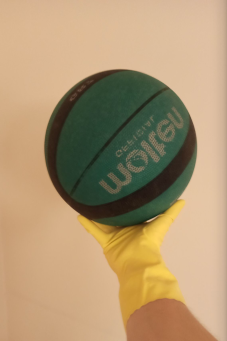
\includegraphics[width=5cm]{img/hand_before_segmentation} }}
	\qquad
	\subfloat[\centering Vaizdas po segmentavimo pagal pirštinės spalvą]{{
\includegraphics[width=5cm]{img/hand_after_segmentation} }}
	\caption{Segmentavimo pavyzdys}
	\label{fig:example}
\end{figure}

\subsubsubsection{Dominančių objektų spalvų rėžiai}
Atliekant bandymus pastebėta, jog net ir naudojantis HSV spalvų erdve, dominančių objektų spalvų rėžiai gan smarkiai keičiasi priklausomai nuo apšvietimo. Šiame darbe naudoti spalvų rėžiai:

\begin{itemize} 
	\item žalsvo kamuolio – nuo [73, 85, 38] iki [85, 230, 180],
	\item geltonų pirštinių – nuo [29,55,130] iki [56,140,255],
	\item raudonų batų – nuo [0,120,255] iki [10,255,200] ir nuo [170,120,255] iki [180,255,200].
\end{itemize}

Tinkamų HSV rėžių radimo procedūra buvo pasirinkus tam tikrą pradinį intervalą patikrinti, ar nufiltravus netinkamus pikselius, išskirtas regiono plotas atitinka dominančio objekto plotą. Jei išskirto regiono plotas yra mažesnis – vadinasi, rėžiai yra per siauri, tad jie buvo didinami, tuo tarpu jei plotas yra didesnis – rėžiai mažinami. 

Šitaip bandymų būdu buvo sukalibruoti paruoštai vaizdo medžiagai labiausiai tinkami spalvų rėžiai. Dėl galimų artifaktų atsiradimo (pvz. triukšmo ar nesusijusių objektų) nufiltravus pikselius pagal spalvos rėžius, buvo bandoma juos turėti kuo siauresnius, tačiau kaip vėliau pasirodė iš rezultatų, net ir menkiausias apšvietimo pokytis turėjo itin didelę įtaką spalvoms. Kiekvienai vaizdo medžiagai, nufilmuotai skirtingose aplinkose, ieškomų spalvų reikšmes gali tekti kalibruoti iš naujo.

Taip pat buvo pastebėta, jog lauke filmuotuose vaizdo įrašuose spalvos kito mažiau, nei kambaryje – tai, galimai, yra geresnio apšvietimo pasekmė. 

\subsubsection{Morfologinės transformacijos}
Atlikus segmentavimą pagal spalvą, rezultate dažnai lieka triukšmo ar bereikalingų artifaktų, kurie gali neigiamai paveikti tolimesnį apdorojimą.

Tokiais atvejais apsivalyti nuo triukšmo gan dažnai naudojamos slenkstinės (\textit{angl.} threshold) operacijos \cite[112]{SzeliskiCompVision}. Apsibrėžus tam tikrą filtrą, jo pagalba matricoje galima atlikti eroziją ir plėstį. Erozija naudojama tada, kai norima sumažinti turimų atskirų regionų paveikslėlyje plotus, nuardant kraštus. Jei objektai yra sąlyginai maži, atlikus erozijos operaciją jie visai išnyksta, taip pašalinant triukšmą. Formaliai erozija buvo aprašyta 1980 metais K. Y. Yoo \cite{4767941} kaip morfologinė operacija, sukombinuojanti dvi aibes naudojant vektorių atimtį aibių elementams. Matematiškai tai apsirašo: 

\begin{equation}\label{eq:erozija}
	A \ominus B = \bigcap_ {b \in B } (A)_{-b} .
\end{equation}

\ref{eq:erozija} lygtyje A žymi dominantį paveikslėlį, išreikštą matrica, o B – filtrą arba kitaip – struktūrinį elementą, su kuriuo A matricoje pakartotinai atliekamos sankirtos.  

Erozijai priešinga operacija yra plėstis \cite{4767941}. Ši operacija leidžia padidinti išskirtų regionų plotą. Plėstis naudinga tuomet, kai po erozijos operacijos objektai praranda per daug ploto. Plėstį galima užrašyti šitaip:

\begin{equation}\label{eq:plestis}
	A \oplus B = \bigcup_ {b \in B } (A)_{b} .
\end{equation}

Atliekant bandymus pastebėta, jog siekiant geriausių rezultatų šalinant triukšmą, plėstį reikėtų vykdyti po erozijos, priešingu atveju triukšmas gali nebūti panaikintas. 

OpenCV įgyvendina funkcijas erode() ir dilate(), kurios priima paveikslėlio matricą ir struktūrinį elementą. Taip pat egzistuoja funkcija morphologyEx(), kuri, priklausomai nuo paduodamų parametrų keičia savo veikimą: su MORPH\_OPEN atliekama plėstis po erozijos, su MORPH\_CLOSE – atvirkščiai. 

\subsubsection{Kamuolio kontūrų radimas}

Siekiant iš paveiksliukų išgauti daugiau kontekstualios informacijos, pavyzdžiui, ar kamuolys yra rankose, išsiskirti tarpusavy nesusikertančius regionus neužtenka. Tam, kad gauti šią informacijos dalį, reikia rasti, kada rankos ir kamuolio regionai susikerta, t.y. jų sankirta yra netuščia. Tam reikia žinoti, kokią erdvę apima kamuolys – šios informacijos trūksta po segmentavimo pagal spalvą, jei kamuolys yra uždengtas, pavyzdžiui, rankos. 

Vienas iš būdų šią problemą išspręsti – pabandyti atspėti, kokią sritį užima kamuolys randant jo kontūrus. Skritulių kontūrams rasti 1991 metais E. Welzl pasiūlė algoritmą, rekursiškai apskaičiuojantį tam tikrai taškų aibei mažiausią ją apimantį apskritimą \cite{Welzl91smallestenclosing}. Šis algoritmas – tiesinio kompleksiškumo, jį įgyvendina OpenCV funkcija minEnclosingCircle().       

\begin{figure}[H]
	\centering
	\subfloat[\centering Kamuolio kontūrai prieš mažiausio aibę apimančio apskritimo radimo algoritmą]{{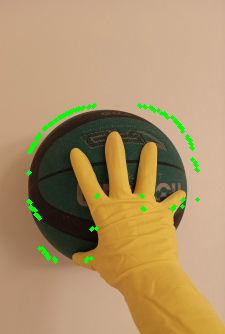
\includegraphics[width=5cm]{img/ball_contours_before} }}
	\qquad
	\subfloat[\centering Kamuolio kontūrai po mažiausio aibę apimančio apskritimo radimo algoritmo]{{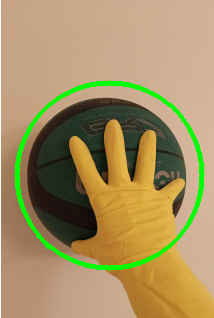
\includegraphics[width=5cm]{img/ball_contours_after} }}
	\caption{Kontūrų radimo algoritmo pavyzdys}
	\label{fig:example}
\end{figure}

\subsection{Atpažinimas remiantis skirtumais}
\subsubsection{Fono pašalinimas}
Fono pašalinimas yra vienas iš esminių metodų kompiuterinėje regoje, naudojamas išskirti dominančius vaizdus ir pašalinti nereikalingus statiškus objektus iš fono. Pavyzdžiui, jei yra filmuojama lauke, fone besimatantys medžiai gali trukdyti tolimesniam atpažinimui, tad žinant, jog mus domina tik žaidėjas, pašalinius objektus galima pabandyti pašalinti. Vienas iš būdų yra iš anksto turėti fono paveiksliuką ir apdorojant kitus kadrus jį išimti, bet tai dažnai nepasiteisina dėl to, kad fonas gali kisti – gali atsirasti šešėlių, pasikeisti apšvietimas, gali būti įvairaus pašalinio judėjimo, pavyzdžiui – linguojantys medžiai, vaikštantys sirgaliai ir pan. 2002 m.  P. KaewTraKulPong pasiūlė algoritmą, išsprendžiantį šią problemą \cite{KaewTraKulPong2002}. Algoritmas kiekvieną pikselį sumodeliuoja į Gauso skirstinį pagal tai, kiek pikselio spalva keičiasi bėgant laikui. Kuo mažiau pikseliai keičiasi, tuo didesnė tikimybė, kad jie priklauso fonui. Naudojantis šiuo atradimu sėkmingai atsikratoma fono, taip išskiriant mus dominantį vaizdą. Šis metodas ypač tinkamas atpažinti judėjimui – vietoje stovintis žaidėjas bus priskirtas fonui, tačiau jam judant, lengvai išskiriamas jo siluetas.  

\begin{figure}[H]
    \centering
    \subfloat[\centering Vaizdas prieš fono pašalinimą.]{{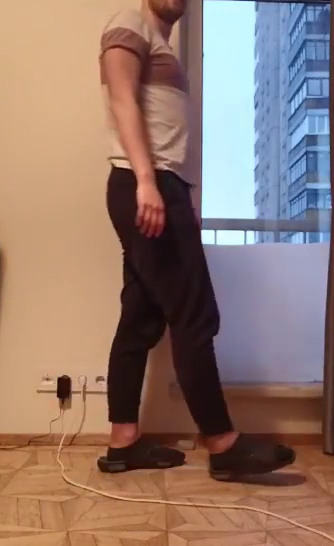
\includegraphics[width=5cm]{img/background-substraction-before} }}
    \qquad
    \subfloat[\centering Vaizdas po fono pašalinimo.]{{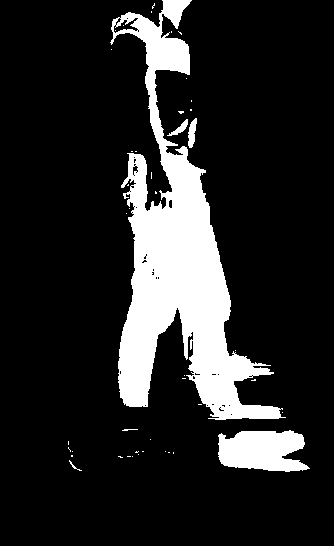
\includegraphics[width=5cm]{img/background-substraction} }}
    \caption{Fono pašalinimas naudojantis Gauso skirstiniu paremtu fono segmentavimo algoritmu}
    \label{fig:example}
\end{figure}


Paveikslėlyje matome, jog algoritmas atpažino žmogaus siluetą. Šiame pavyzdyje ranka priskirta fonui dėl to, jog spalva sutampa su sienos spalva, tačiau kitos kūno dalys išskiriamos iš fono.

\subsubsection{Judesio atpažinimas}\label{section:movement}

Žaidėjui vaikštant, kai kurios kūno dalys juda greičiau, nei kitos. Kūnas išlieka santykinai statiškas palyginus su kojomis. Žingsniavimo mechanika yra tokia, kad atliekant žingsnį, viena koja lieka vienoje vietoje, kol kita yra perstatoma iš vienos pozicijos į kitą. Tam, kad pagauti tą kojos judesį, iš antrojo kadro atimamas pirmasis. Padalijus kadrą į dvi dalis – viršutinę ir apatinę – ir darant prielaidą, jog apatinėje dalyje matysis tik kojų judesiai, galima teigti, kad jei atėmus antrą kadrą iš pirmo yra skirtumas, buvo atliktas žingsnis. Koją pastačius ant žemės, tam tikrą laiką skirtumai sumažėja iki nustatytos ribos – pasinaudojus visa šia informacija galima apskaičiuoti, kiek žingsnių buvo atlikta. 

\begin{figure}[H]
    \centering
    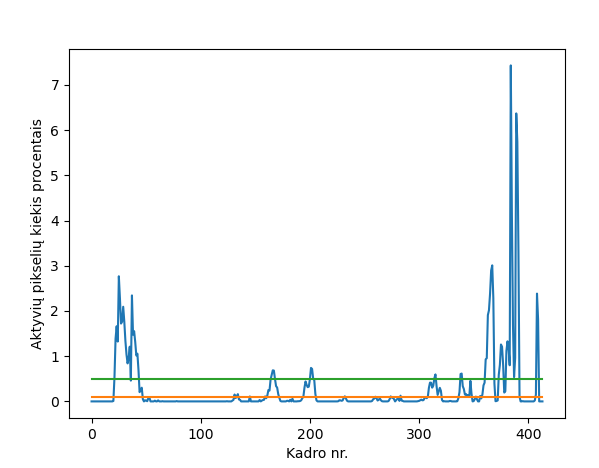
\includegraphics[scale=0.8]{img/steps}
    \caption{Aktyvių pikselių kiekis kiekviename kadre, indikuojantis žmogaus judėjimą }
    \label{img:steps}
\end{figure}

\ref{img:steps} paveikslėlyje matyti, kiek buvo aktyvių pikselių kiekvieną kadrą panaudojus fono pašalinimą bei kadrų skirtumo algoritmus. Ši informacija rodo judėjimo kiekį tam tikrame kadro regione. Žalia linija žymi minimalų judėjimo kiekį, kuris gali atsirasti dėl triukšmo ir pašalinio judėjimo. Viršijus šią liniją galima teigti, jog žaidėjas šiuo metu juda. Oranžinė linija žymi ribą, iki kurios galima sakyti, jog jokio judesio nėra, t.y. žaidėjas pastatė koją ir ruošiasi atlikti kitą žingsnį. 

\subsection{Žmogaus kūno dalių atpažinimas neuroniniais tinklais}

Šiuolaikinėje kompiuterinės regos srityje daug naudos galima gauti pasinaudojus neuroninių tinklų pagalba. Neuroniniai tinklai naudojami sprendžiant įvairias problemas, šiam darbui aktualiausia yra objektų atpažinimo problema. Turint tam tikrą kadrą, taisyklių pažeidimo algoritmui būtina, kad būtų atskirtos rankos, kojos ir kamuolys. Žmogaus kūno dalių klasifikavimas yra sudėtinga problema, kadangi dauguma algoritmų yra priklausomi nuo surinktų duomenų. Kompleksija tampa akivaizdi sprendžiant sporto problemas, kadangi labai dažnai žaidėjai daro įvairiausius judesius, apsirengę įvairiausiais rūbais ir pan., kas apsunkina žaidėjo kūno dalių atpažinimą \cite{Andriluka_2014_CVPR}. Tam reikalinga turtinga ir didelė duomenų aibė, dėl ko neuroninio tinklo apmokymo laikas išauga. 

Bene visi šiuolaikiniai metodai remiasi tuo pačiu principu: apmokinamas neuroninių tinklų modelis, jiems paruošiant teigiamus ir neigiamus pavyzdžius (pvz., siekiant sukurti kojų atpažinimo algoritmą, paveiksliukai, kuriuose yra koja pažymimi kaip teigiami, tie, kuriuose kojos nėra tampa neigiamais). Mokinimo procesas gali trukti daug laiko – kartais net savaites, todėl daug paprasčiau yra pasinaudoti jau sukurtu modeliu. Vienas iš modelių, pavadinimu OpenPose, buvo pasiūlytas 2018 metais \cite{cao2019openpose}. Modelio architektūra paremta konvoliuciniais neuroniniais tinklais. Modelis suskirstytas į dvi šakas. Viena jų priskiria tikimybes, kad tam tikras regionas yra tam tikra kūno dalis, kita – asociacijas tarp skirtingų kūno dalių. Atpažinimas vyksta keliais etapais, siekiant gauti kuo tikslesnius rezultatus. 

Šiame darbe kuriamas vaizdo atpažinimo algoritmas kiekvieną kadrą pateikia neuroniniui tinklui, kuris apskaičiuoja ir grąžina šiluminį žemėlapį (\textit{angl.} heatmap) su sąnarių koordinatėmis ir tikimybėmis, kad tose koordinatėse jas galima rasti. Vėlesnis apdorojimas pagal grąžintas koordinates kadre skirtingomis spalvomis sužymi dominančias kūno dalis, aplink gautas koordinates nupiešiant fiksuoto spindulio ir spalvos skritulį. Taisyklių pažeidimo atpažinimo algoritmui aktualios yra rankų ir pėdų sritis. Verta pabrėžti, jog randamos yra sąnarių pozicijos, ir nuo algoritmo priklauso, ar tokia informacija yra pakankamai tiksli. 

\begin{figure}[H]
    \centering
    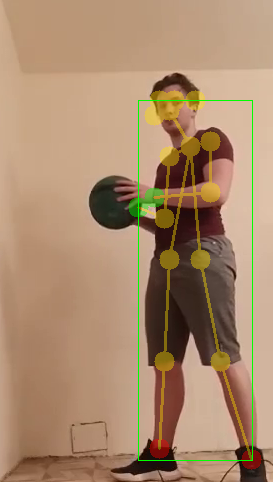
\includegraphics[scale=0.8]{img/body-parts-better}
    \caption{OpenPose algoritmo pagalba atpažintos kūno dalys}
    \label{img:mlp}
\end{figure}

Vienas iš algoritmo trūkumų yra tai, kad be optimizavimo su kiekvienu kadru gauti rezultatą užtrunka iki 0.5 sekundės. Galimas optimizavimo būdas yra sumažinti kadro dydį prieš pateikiant jį į neuroninį tinklą, tačiau tuomet proporcingai mažėja ir tikslumas. 

2018 m. buvo pasiūlytas OpenPose modelio patobulinimas, įgalinantis žmogaus kūno atpažinimą beveik realiu laiku \cite{osokin2018realtime}. Lightweight optimizuoja OpenPose modelio architektūrą sumažinant sluoksnių skaičių, ryškiai pagerinant atpažinimo greitį nežymiai prarandant tikslumą. 

Atliekant bandymus su vaizdo medžiaga pastebėta, jog Lightweight modelis žaidėjo pozą atpažįsta ne tik greičiau, bet ir tiksliau. Eksperimentui buvo sukurti penki vaizdo įrašai, kuriuose žmogus atlieka tam tikrus veiksmus. Tikslumas buvo apskaičiuotas už teisingą kūno dalies atpažinimą kiekviename kadre pridedant 1 tašką, už neteisingą atpažinimą atimant 1, o gautą rezultatą padalinant iš kūno dalių skaičiaus, kurį atpažįsta modelis.

\begin{table}[H]\footnotesize
	\centering
	\caption{OpenPose ir Lightweight modelių palyginimimas apdorojant vienodus vaizdo įrašus}
	{\begin{tabular}{|c|c|c|} \hline
			\textbf{Modelis} & \textbf{Vidutinė trukmė apdoroti vieną kadrą (ms)} & \textbf{Vidutinis rezultatų tikslumas (\%)} \\
			\hline
			OpenPose  & 581    & 62       \\
			\hline
			Lightweight  & 163    & 91       \\
			\hline
	\end{tabular}}
	\label{tab:openposevslightweight}
\end{table}

Dalį Lightweight modelio tikslumo pranašumo galėjo lemti OpenPose parametrų ir paduodamo kadro dimensijų neatitikimas, o spartumo – tai, jog duomenų apskaičiavimas OpenPose tinklu buvo įgyvendintas su OpenCV dnn moduliu, kuris bandymų metu nebuvo sukonfigūruotas naudoti GPU akceleravimą. Kadangi po optimizacijos Lightweight modelis tenkino tikslumo ir greičio lūkesčius, toliau naudoti nuspręsta jį. 

\subsubsection{Atpažinimo neuroniniais tinklais optimizavimas}

Atliekant bandymus pastebėta, jog atpažinimą Lightweight modeliu galima optimizuoti. Viena iš optimizacijų, kuri buvo atlikta, tai skaičiavimo naštos perkėlimas ant GPU. Tam panaudota CUDA – NVIDIA sukurtas API paraleliems skaičiavimams \cite{cuda}. Integravus OpenCV su CUDA, paveikslėlių apdorojimas gali pagreitėti iki 30 kartų \cite{opencv-cuda}. Be GPU akceleracijos Lightweight tinklas vieną kadrą užtrukdavo apdoroti iki 680 ms. 

Pastebėta, jog apdorojimo greičiui įtakos turi ir kadro dimensijos. Jei į neuroninį tinklą paduodamo kadro plotis yra didesnis, nei jo aukštis, apdorojimo greitis pakyla iki 5 kartų. Tačiau tai buvo mitiguota atnaujinus OpenCV versiją iš 4.0.1 į 4.5.1 – po šio atnaujinimo, apdorojimo greičiai tapo nebepriklausomi nuo santykio tarp paveikslėlio aukščio ir pločio. 

Dar viena išbandyta optimizacija – neuroninio tinklo pradinio sluoksnio įvesties dydžio sumažinimas. Dvigubai sumažinus įvesties kanalų skaičių iš 256 į 128 rezultatų tikslumas pasikeitė sąlyginai nedaug. Žiūrint į vaizdo įrašą, plika akimi galima pamatyti, jog atpažintas skeletas yra labiau „klibantis“, t.y. kiekvienos kūno dalies koordinatės nežymiai skiriasi, kai įvesties dydis yra mažesnis, tačiau pačios kūno dalys dažnai lieka atpažintos teisingai. Siekiant tikslesnių rezultatų, siūloma pasilikti prie 256 kanalų skaičiaus, tačiau norint vaizdą apdoroti realiu laiku, galima rasti kompromisą tarp tikslumo ir greičio. 

Atliekant žmogaus skeleto atpažinimo bandymus su mažesnės rezoliucijos kadrais spartumo bei tikslumo pagerėjimų nepastebėta.

\begin{table}[H]\footnotesize
	\centering
	\caption{Lightweight optimizavimas sumažinus įvesties kanalų skaičių apdorojant vienodus vaizdo įrašus}
	{\begin{tabular}{|c|c|c|} \hline
			\textbf{Kanalų skaičius} & \textbf{Vidutinė trukmė apdoroti vieną kadrą (ms)} & \textbf{Vidutinis rezultatų tikslumas (\%)} \\
			\hline
			256  & 28    & 91       \\
			\hline
			128  & 16    & 86       \\
			\hline
	\end{tabular}}
	\label{tab:openposevslightweight}
\end{table}

\subsection{Kamuolio atpažinimas Hough transformacija}

Kompiuterinės regos srityje vieni iš pirmųjų algoritmų, skirtų atpažinti objektus pagal jų formas, yra Hough transformacijos.
Hough transformacija paremtas algoritmas, skirtas skritulių bei apskritimų radimui, buvo aprašytas H. K. Yuen, J. Princen, J. Illingworth ir kitų \cite{YUEN199071}. Būtent šį algoritmą OpenCV įgyvendina kaip numatytąjį, bandant rasti apskritimų kontūrus paveikslėliuose.

Patikrinus algoritmą su vaizdo įrašu tapo akivaizdu, jog šis jis tinka tik idealios formoms sferoms ir apskritimams, tačiau judėdamas kamuolys praranda apvalią formą. Darant prielaidą, jog tokiu atveju kamuolio forma tampa panaši į elipsės, kamuolio radimui išbandytas Hough transformacija paremtas algoritmas elipsėms rasti \cite{1048464}, tačiau šio algoritmo sparta pasirodė itin prasta – atlikus bandymus su keliais vaizdo įrašais, vienam kadrui apdoroti užtrukdavo iki 10 minučių.

\begin{figure}[H]
	\centering
	\subfloat[\centering Atrastas kamuolys]{{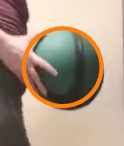
\includegraphics[width=5cm]{img/ball_circled} }}
	\qquad
	\subfloat[\centering Kamuolys nerastas, kadangi jis deformuotas dėl judėjimo]{{
\includegraphics[width=5cm]{img/ball_notfound} }}
	\caption{Kamuolio kontūrų radimas}
	\label{fig:contours}
\end{figure}

Dėl šių trūkumų tolimesniam vaizdo atpažinimui nuspręsta taikyti kamuolio atpažinimo pagal spalvą metodus, kadangi preliminarūs rezultatai parodė, jog kadrus apdoroti spalviniu atpažinimu paremtais algoritmais užtrunka šimtus kartų mažiau laiko, nei elipsių paieškos algoritmas, taip pat – jie yra tikslesni, pasirinkus teisingus spalvos rėžius. 

\subsection{Nagrinėtų atpažinimo metodų palyginimas}

Tam, kad būtų palygintas šių metodų spartumas bei tikslumas tarpusavy, nuspręsta juos panaudoti sprendžiant praktinę problemą: vaizdo įraše suskaičiuoti, kiek žmogus atliko žingsnių. Žingsnių skaičiavimo algoritmas – gana paprastas, nereikalaujantis daug papildomų sudėtingų skaičiavimų, tad jis puikiai tinka įvertinti pačio vaizdo atpažinimo metodo tinkamumą.  

Žingsnių skaičiavimo algoritmas yra žingsnių taisyklės pažeidimo atpažinimo dalis, plačiau apibūdintas 4 skyriuje. Žmogaus skeleto (pozos) bei spalvinio atpažinimo metodai įgyvendinti tuo pačiu algoritmu, kurio metu pėdų (batų) regionai yra išskiriami, ir laikoma, jog žingsnis yra atliktas tada, kai išskirti regionai persikloja – tai reiškia, jog žiūrint iš šono, įprasto vaikščiojimo metu viena koja trumpai pridengė kitą. Neuroninių tinklų atpažinimo metu prie atpažintų kojų priskiriamos spalvos, tolimesnis atpažinimas panašus į spalvinį.

Metodo, besiremiančio skirtumais tarp kadrų, žingsnių atpažinimo procesas aprašytas 3.2.2 poskyryje.

Visuose vaizdo įrašuose žmogus dėvi raudonus batus, tam, kad veiktų spalvomis paremti atpažinimo metodai ir juos būtų galima lyginti su kitais. Vaizdo įrašų sukurta septyni, juose – skirtingas apšvietimas, nuotolis iki žmogaus, žingsniai atliekami skirtingu tempu ir kamera filmuoja skirtingais kampais. 

Algoritmai buvo patikrinti kelis kartus su tais pačiais įrašais, siekiant sumažinti įvairių kitų kompiuteryje vykstančių procesų įtaką vaizdo apdorojimo greičiui. 

\begin{table}[H]\footnotesize
	\centering
	\caption{Vaizdo įrašai ir jų aprašymai}
	{\begin{tabular}{|p{2cm}|p{8cm}|p{2cm}|} \hline
			\textbf{Vaizdo įrašo nr.} & \textbf{Aprašymas}  & \textbf{Trukmė (s)} \\
			\hline
			1  & Besikeičiantis apšvietimas, žaidėjas eina įstrižai nuo kameros, vaizdo įrašas filmuotas vertikaliai & 12      \\
			\hline
			2  & Žaidėjas eina atgal, kamera filmuoja iš priekio, filmuota horizontaliai          & 2 \\
			\hline
			3  & Žaidėjas vaikšto gan tolokai nuo kameros, filmuota horizontaliai       	 & 5 \\ 
			\hline
			4  & Žaidėjas labai arti kameros, filmuota horizontaliai       
		 	& 7  \\ \hline
			5  & Žaidėjas vaikšto gan tolokai nuo kameros, filmuota vertikaliai, žaidėjas matomas pilnai    & 8    \\
			\hline
			6  & Prastas apšvietimas, žaidėjas gan arti kameros, filmuota horizontaliai       
			& 8 \\
			\hline
			7  & Žaidėjas toli nuo kameros, atsiranda antras žaidėjas, filmuota horizontaliai. Tikimasi, kad bus suskaičiuota abiejų žaidėjų žingsnių suma   & 10     \\
			\hline
	\end{tabular}}
	\label{tab:openposevslightweight}
\end{table}


\begin{table}[H]\footnotesize
	\centering
	\caption{Spalvinio vaizdo atpažinimo žingsnių skaičiavimo eksperimento rezultatai}
	{\begin{tabular}{|p{3cm}|p{3cm}|p{3cm}|p{3cm}|} \hline
			\textbf{Vaizdo įrašo nr.} & \textbf{Atlikta žingsnių} & \textbf{Algoritmo suskaičiuota žingsnių} & \textbf{Vidutinė vaizdo apdorojimo trukmė (ms)} \\
			\hline
			1  & 10    & 13    & 6035    \\
			\hline
			2  & 3    & 0  & 4681     \\
			\hline
			3  & 4    & 2   & 12600    \\
			\hline
			4  & 7    & 7  & 4126     \\
			\hline
			5  & 5    & 5  & 4029     \\
			\hline
			6  & 7    & 6  & 3949     \\
			\hline
			7  & 10    & 6  & 4235     \\
			\hline
	\end{tabular}}
	\label{tab:colorresults}
\end{table}

\begin{table}[H]\footnotesize
	\centering
	\caption{Vaizdo atpažinimo pagal skirtumus žingsnių skaičiavimo eksperimento rezultatai}
	{\begin{tabular}{|p{3cm}|p{3cm}|p{3cm}|p{3cm}|} \hline
			\textbf{Vaizdo įrašo nr.} & \textbf{Atlikta žingsnių} & \textbf{Algoritmo suskaičiuota žingsnių} & \textbf{Vidutinė vaizdo apdorojimo trukmė (ms)} \\
			\hline
			1  & 10    & 9    & 4807    \\
			\hline
			2  & 3    & 4  & 5488     \\
			\hline
			3  & 4    & 4   & 11529    \\
			\hline
			4  & 7    & 10  & 2164     \\
			\hline
			5  & 5    & 2  & 3147     \\
			\hline
			6  & 7    & 8  & 3012     \\
			\hline
			7  & 6    & 4  & 3983     \\
			\hline
	\end{tabular}}
	\label{tab:diffresults}
\end{table}

\begin{table}[H]\footnotesize
	\centering
	\caption{Vaizdo atpažinimo su neuroniniais tinklais žingsnių skaičiavimo eksperimento rezultatai}
	{\begin{tabular}{|p{3cm}|p{3cm}|p{3cm}|p{3cm}|} \hline
			\textbf{Vaizdo įrašo nr.} & \textbf{Atlikta žingsnių} & \textbf{Algoritmo suskaičiuota žingsnių} & \textbf{Vidutinė vaizdo apdorojimo trukmė (ms)} \\
			\hline
			1  & 10    & 8    & 12859    \\
			\hline
			2  & 3    & 0  & 7196     \\
			\hline
			3  & 4    & 4   & 14565    \\
			\hline
			4  & 7    & 0  & 1257     \\
			\hline
			5  & 5    & 5  & 11638     \\
			\hline
			6  & 7    & 8  & 12438     \\
			\hline
			7  & 6    & 6  & 10045     \\
			\hline
	\end{tabular}}
	\label{tab:poseresults}
\end{table}

Palyginę rezultatus matome, jog neuroniniais tinklais paremtas atpažinimas yra tiksliausias, nors ir apdoroti vaizdo įrašą užtrunka daugiausiai laiko. Atpažinimas remiantis skirtumais – greičiausias, tačiau mažiausias yra jo tikslumas, o atpažinimas paremtas spalvomis yra per vidurį. 

Spalvomis paremtas atpažinimas yra mažiausiai tikslus, kai varijuoja apšvietimas arba jis yra prastas, taip pat – jei kadre yra kitų objektų ar žaidėjų, kurių spalvos sutampa su dominančiomis spalvomis. Taip pat šiuo atpažinimu paremtas algoritmas vienintelis, galintis apskaičiuoti žaidėjo atliktus žingsnius iš priekio. 

Iš rezultatų apdorojant vaizdo įrašą nr. 4 pastebima, jog neuroniniais tinklais paremtas atpažinimo metodas neatpažįsta žingsnių, kai žaidėjas yra per arti kameros ir nebesimato jo pilnos figūros, tuo tarpu vaizdo įrašas nr. 7 parodo, jog šis atpažinimo metodas puikiai susidoroja su atvejais, kai yra daugiau žmonių, nei vienas. 

Apibendrinus – spalviniai vaizdo atpažinimo metodai tinka tuomet, kai prie dominančių objektų galime priskirti unikalias spalvas, jos nekinta, neatsiranda naujų, o apšvietimas išlieka puikus – visa tai indikuoja, jog vaizdo įraše fonas ir aplinka turi būti griežtai kontroliuojami ir iš anksto paruošti. Skirtumais paremti atpažinimo metodai labiausiai tinka tais atvejais, kai juos naudojantys algoritmai yra paprasti bei nereikalaujantys didelio tikslumo, siekiant išgauti didžiausią spartumą. Neuroniniais tinklais paremti atpažinimo metodai yra itin tikslūs, tačiau apdorojimo trukmė yra šiek tiek ilgesnė.

\section{Krepšinio taisyklių pažeidimo atpažinimas}

Šiame skyriuje bus aprašomi algoritmai žingsnių bei dvigubo varymo taisyklių atpažinimui.

\subsection{Žingsnių taisyklė}
Žingsnių (\textit{angl.} traveling) taisyklė yra aprašyta oficialioje NBA taisyklių knygelės 10 taisyklės 13 skyriuje. Jos formuluotė, kuria remiasi analizė, atlikta šiame darbe, yra tokia: 

\begin{itemize}
	\item Žaidėjas, varydamas kamuolį, gali padaryti du žingsnius prieš sustojant arba kamuolį metant ar atiduodant \cite{nba-rules}. 
\end{itemize}

Taisyklių knygelėje yra aprašyti keletas veiksmų, pažeidžiančių taisyklę (pavyzdžiui, ėjimas gavus kamuolį jo bent kartą nesumušant ar atraminės kojos pakėlimas sustabdžius varymą), tačiau šiame darbe fokusuojamasi į atvejį, kai žaidėjas suėmęs kamuolį atlieka daugiau nei du žingsnius. Tam, kad atlikti žingsniai būtų laikomi kaip pažeidžiantys taisyklę, kamuolys turi būti nemušamas į žemę, o laikomas rankose – krepšinyje tai dažniausiai nutinka prieš metant kamuolį į krepšį, kai yra atliekamas dvižingsnis. Taigi, algoritmas, siekiantis atpažinti šios taisyklės pažeidimą, privalo taip pat gebėti atpažinti, kada kamuolys yra rankose, ir tuomet skaičiuoti atliktų žingsnių skaičių. 

\subsection{Žingsnių taisyklės pažeidimo atpažinimo algoritmas}

Algoritmo reikalavimai yra nustatytos rankų, kojų bei kamuolio vietos paveikslėlyje. Apibendrintas algoritmas užsirašytų šitaip: 

\begin{enumerate}
	\item nuskaitomas kadras,
	\item nustatoma, ar kamuolys yra laikomas rankose,
	\item tol, kol kamuolys yra rankose, vykdomas žingsnių skaičiavimo algoritmas,
	\item jei per intervalą, kai kamuolys yra laikomas rankose, buvo atlikti daugiau nei 2 žingsniai – grąžinamas rezultatas, jog taisyklė pažeista.
\end{enumerate}

\begin{figure}[H]
	\centering
	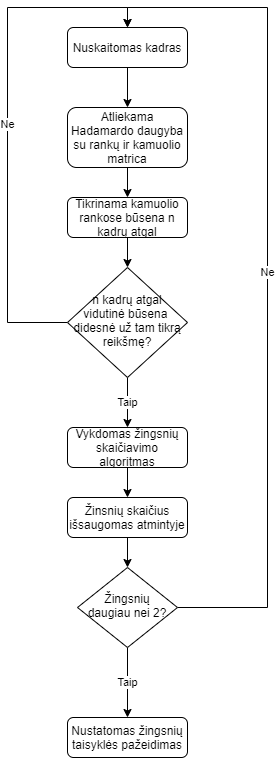
\includegraphics[scale=0.6]{img/travel_algorithm}
	\caption{Žingsnių taisyklės pažeidimo atpažinimo algoritmas}
	\label{img:travel_algo}
\end{figure}

Algoritmui vienas po kito pateikiami vaizdo įrašo kadrai, kurie yra apdorojami po vieną. Po anksčiau aprašytų atpažinimo metodų turima pakankamai informacijos nustatyti, kur kiekviename kadre yra ranka, kojos ir kamuolys. OpenCV įgalina visų minėtųjų metodų metu išgautą informaciją reprezentuoti loginėse vienetų bei nulių matricose, kur vienetai žymi objekto buvimą tam tikrame plote. 

Tam, kad būtų nustatyta, ar kamuolys yra laikomas rankose, su išskirtomis kamuolio ir rankų užimamą erdvę kadre reprezentuojančiomis loginėmis matricomis atliekama Hadamardo daugyba, t.y. kiekvienam matricos elementui atliekama disjunkcija su toje pačioje vietoje esančiu elementu iš kitos matricos.

Spalvinio atpažinimo metodų sukurtos matricos yra pačių kūno dalių projekcija, tačiau naudotas neuroninių tinklų modelis grąžina apytikslias sąnarių koordinates (riešo, kulkšnies), aplink kuriuos nupiešiamas skritulys – iš to galima spręsti, kur maždaug yra ranka ar pėda.  

Rezultate gaunama matrica, žyminti sritį, kur rankos bei kamuolys persikloja. Tai reiškia, jog kamuolio ir rankų pozicija kadre sutampa, tačiau tam tikra rankos dalis yra arčiau kameros ir šiek tiek užstoja kamuolį. 

\begin{figure}[H]
	\centering
	\subfloat[\centering Ranka]{{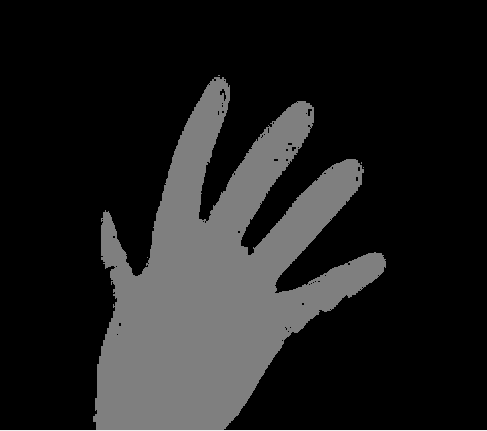
\includegraphics[width=5cm]{img/hand.png} }}
	\qquad
	\subfloat[\centering Kamuolys]{{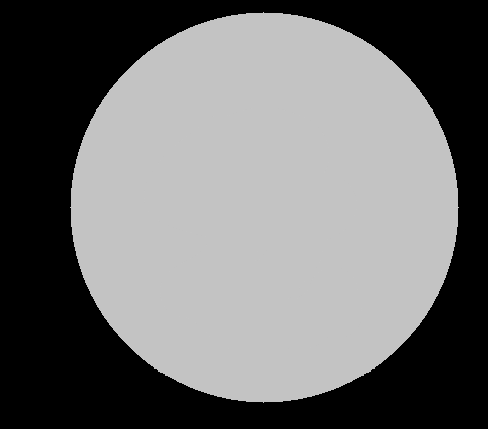
\includegraphics[width=5cm]{img/ball.png} }}
	\qquad
	\subfloat[\centering Ranka arba kamuolys]{{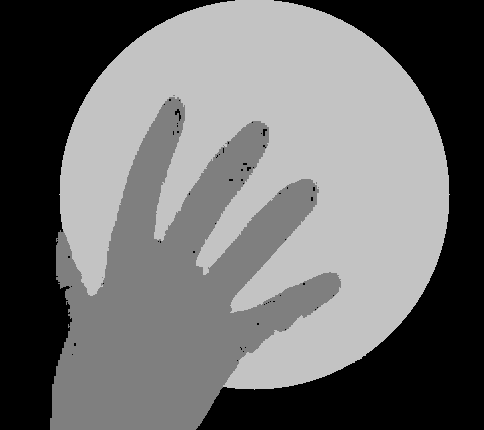
\includegraphics[width=5cm]{img/hand_or_ball.png} }}
	\qquad
	\subfloat[\centering Ranka ir kamuolys (Hadamardo daugyba)]{{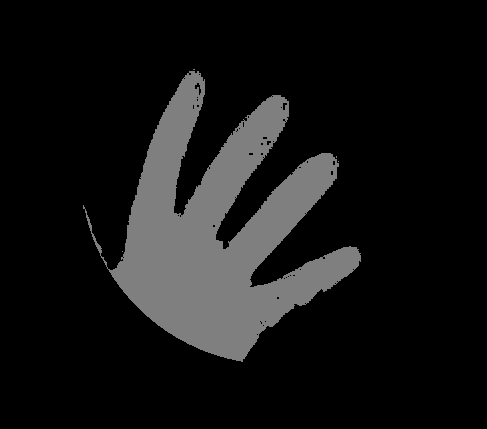
\includegraphics[width=5cm]{img/hand_and_ball.png} }}
	\caption{Kamuolio ir rankų santykio nustatymas}
	\label{fig:hand_and_ball}
\end{figure}

\subsection{Žingsnių skaičiavimo algoritmas}

Šiek tiek sunkiau apibrėžti universalų būdą atpažinti atliktus žingsnius iš bet kokio kampo. Paprastumo dėlei nuspręsta žingsnius skaičiuoti tik žiūrint iš šono. Žingsnių skaičiavimo algoritmas remiasi išskirtų kojų regionų kontūrų skaičiavimu. Jei kontūrų suskaičiuojama vienas, kai prieš tai jų buvo du, galima teigti kad: 1) nerasta informacijos apie vieną iš pėdų (išėjo iš kadro arba nepavyko atpažinimas) arba 2) žingsnis, žiūrint iš šono, yra toje fazėje, kai viena pėda pridengia (arba yra netoli) kitą. Tam, kad būtų galima atmesti pirmąjį atvejį, laikoma informacija apie atpažintus objektus – jei jų yra vienas, tuomet tai, kad rastas tik vienas kontūras, nekeičia turimų suskaičiuotų žingsnių kiekio. 

\begin{figure}[H]
	\centering
	\subfloat[\centering Žingsnio pradžia, randami du kontūrai]{{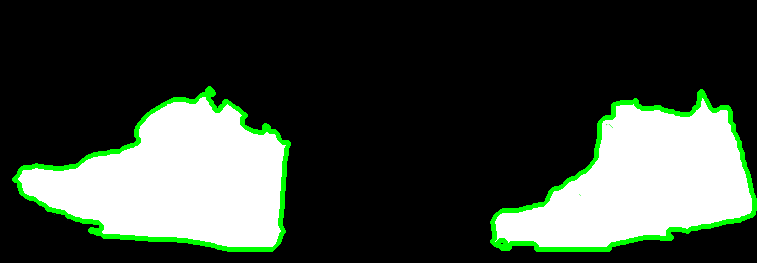
\includegraphics[width=5cm]{img/step_contours1.png} }}
	\qquad
	\subfloat[\centering Žingsnis tęsiasi, kontūrai vis dar du]{{
\includegraphics[width=5cm]{img/step_contours2.png} }}
	\qquad
	\subfloat[\centering Įpusėjęs žingsnis, kontūrai susilieja į vieną]{{
\includegraphics[width=5cm]{img/step_contours3.png} }}
	\caption{Žingsnio atpažinimo procesas skaičiuojant kontūrus}
	\label{fig:steps_contours}
\end{figure}


Žingsnių skaičiavimo algoritmą, kuris taikytinas reikiamą informaciją išgavus spalviniais atpažinimo metodais arba neuroninių tinklų pagalba, galima apibrėžti taip:

\begin{enumerate}
	\item Išskiriami kojų (batų) regionai.
	\item Suskaičiuojami kontūrai.
	\item Jei kontūrų yra daugiau nei vienas – pasižymima, jog sankirta neįvyko. 
	\item Jei kontūras yra vienas, sankirta dar nebuvo įvykus ir išskirtų regionų skaičius yra daugiau, nei vienas – pasižymima, jog sankirta įvyko ir padidinamas žingsnių skaičius. 
\end{enumerate}

\begin{figure}[H]
	\centering
	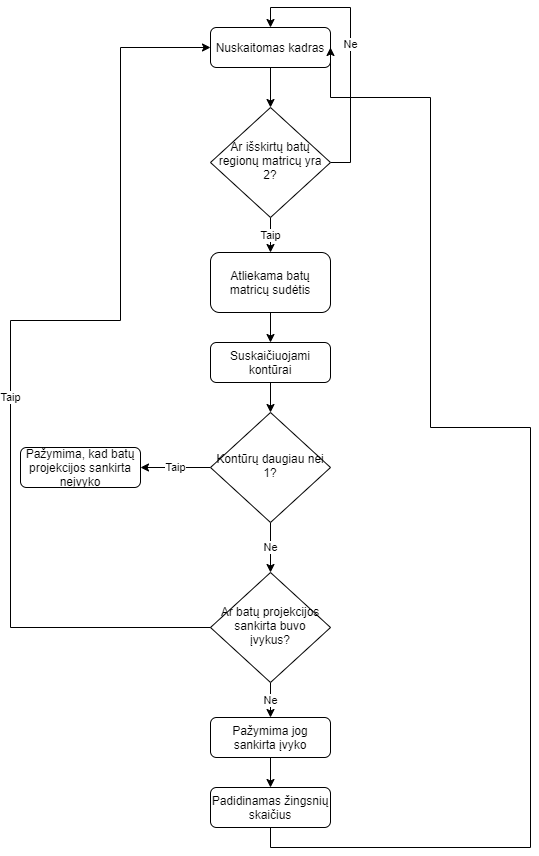
\includegraphics[scale=0.6]{img/steps_algorithm}
	\caption{Žingsnių skaičiavimo algoritmas}
	\label{img:steps_algo}
\end{figure}

Šis žingsniavimo atpažinimo metodas taikytinas tik tada, kai žingsnis yra kiek galima labiau natūralus, t.y. kojos nėra keliamos per aukštai ir pėdos įpusėjus atliekamam žingsniui yra netoli viena kitos. Lankstesnis yra skirtumais tarp kadrų paremtas algoritmas, atpažįstantis, kada atliktas bet koks judėjimas, tačiau jo tikslumas yra prastas.

Turint informaciją apie kamuolio laikymą tam tikrame laiko intervale ir per jį atliktų žingsnių kiekį, galime daryti išvadą, kad žingsnių taisyklė yra pažeista, kai per minėtą intervalą yra atlikti daugiau nei 2 žingsniai. 

\subsubsection{Būsenos saugojimas}
Atliekant pradinius bandymus su algoritmu pastebėta, jog nustatant, ar kamuolys yra rankose, išskirtų rankų bei kamuolio regionų plotai yra nepastovūs priklausomai nuo apšvietimo ir kitų faktorių. Tai reiškia, jog laiko intervalas, kada kamuolys yra laikomas rankose, gali būti su trūkiais, indikuojančiais, kad tą laiko momentą nepavyko nustatyti, ar kamuolys yra rankose. Žingsnių skaičiavimo algoritmas skaičiuoja žingsnius tik tada, kai kamuolys yra rankose, tad intervalui nutrūkus dėl netikslaus atpažinimo, skaičiavimas prasidės iš naujo. 

Informacija apie kamuolio buvimą rankose yra renkama ne iš vieno kadro, o iš kelių, ir darant prielaidą, jog rankose esančio kamuolio judėjimo greitis yra arti nulio, galima teigti, jog tokia būsena turėtų nepasikeisti tam tikrą skaičių kadrų. Kitaip tariant, su kiekvienu kadru išsaugoma būsena, ar kamuolys yra rankose ar ne.

\begin{figure}[H]
	\centering
	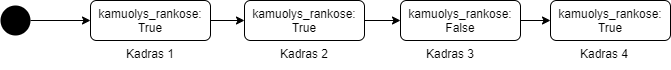
\includegraphics[scale=0.6]{img/state}
	\caption{Būsenos saugojimo pavyzdys kiekviename kadre}
	\label{img:state}
\end{figure}

Išsaugojus būseną suskaičiuojama, kokia buvo jos vidutinė reikšmė per pastaruosius n kadrų: 

\begin{equation}\label{eq:avg_state}
	M_{\textit{vid. būsena}} = \sum_{n=i-x}^{i} \frac{S(n)}{n},
\end{equation}
kur \textit{i} žymi einamo kadro numerį, \textit{x} – konstantą, nurodančią dominančių kadrų skaičių, \textit{S} – \textit{n}-tojo kadro būseną, kur 1 indikuoja kamuolio buvimą rankose, o 0 – atvirkščiai.

Jei vidutinė būsena yra didesnė už tam tikrą iš anksto nustatytą konstantą, pvz., 0.3, galima teigti, jog kamuolys vis dar yra rankose – tam, kad ši reikšmė pasikeistų, turi praeiti bent keli kadrai, pakeičiantys būsenos vidurkį. 

Šis būsenos skaičiavimo būdas atliekant pradinius bandymus su programinės įrangos kodu pasirodė gana naudingas siekiant sumažinti įvarius būsenų svyravimus, kylančius iš atpažinimo netikslumo, tad jis taip pat yra įgyvendintas ir kitame taisyklės pažeidimo algoritme. 

\subsection{Dvigubo varymo taisyklė}
Pagal NBA taisyklių knygelės 10 taisyklės 2 skyriaus c dalį, žaidėjas negali tęsti kamuolio varymo jei jį pats sustabdė. Scenarijai, kada varymas laikomas sustabdytu, aprašyti 4 taisyklės 2 skyriuje. Varymas sustoja, kai kamuolys yra suimamas abejomis rankomis, atiduodamas kitam žaidėjui, metamas į krepšį ar prarandamas kuriuo nors kitu būdu. 

Žaidėjas varymą gali tęsti jei kamuolį atidavus komandos draugui jis buvo grąžintas atgal, taip pat jei po metimo į krepšį žaidėjas pats kamuolį atsikovoja. Visus taisyklei aktualius varymo sustabdymo scenarijus galima supaprastinti į vieną: kamuolys yra suimamas abejomis rankomis. Tam įvykus, žaidėjas gali tik atiduoti kamuolį, mesti į krepšį arba laukti, kol pasibaigs atakai skirtas laikas. 

Taisyklės pažeidimo atpažinimo algoritmas turi atpažinti, jog varymas yra sustojęs, taip pat nustatyti, kada kamuolys buvo išmestas iš rankų ir vėl pagautas (pvz. atliekant varymą antrą kartą). Paprastumo dėlei kuriant algoritmą priimta, jog situacija, kai sustabdžius varymą kamuolys yra išmetamas į orą ir vėl pagaunamas yra taisyklės pažeidimas – tokį veiksmą iš algoritminio atpažinimo perspektyvos sunku atskirti nuo pasavimo ar metimo į krepšį dėl tikslesnių apibrėžimų trūkumo bei subjektyvumo vertinant veiksmo intenciją. Panašus scenarijus apibūdinamas NBA taisyklių 13 skyriuje – žaidėjas metęs ar atidavęs kamuolį negali jo paliesti nepažeidęs taisyklės, jei kamuolio prieš tai nepalietė komandos draugas, priešininkas ar kamuolys neatsimušė nuo lentos ar lanko. Taigi, sustabdžius varymą, kamuolio pagavimas jį išmetus aukštyn ar žemyn yra laikytinas kaip pažeidžiantis taisykles. 

\subsection{Dvigubo varymo taisyklės atpažinimo algoritmas}

Šiam algoritmui, kaip ir žingsnių taisyklės atpažinimo algoritmui, būtina sąlyga – informacija apie kojų (pėdų), kamuolio ir rankų padėtį kadre. Supaprastinta algoritmo versija atrodo taip: 

\begin{enumerate}
 	\item nuskaitomas kadras,
 	\item nustatoma, ar varymas yra sustabdytas,
 	\item nustatoma, ar kamuolys yra išmetamas iš rankų,
 	\item jei kamuolys yra žaidėjo vėl pagaunamas, grąžinama, kad taisyklė yra pažeista.
\end{enumerate}

\begin{figure}[H]
	\centering
	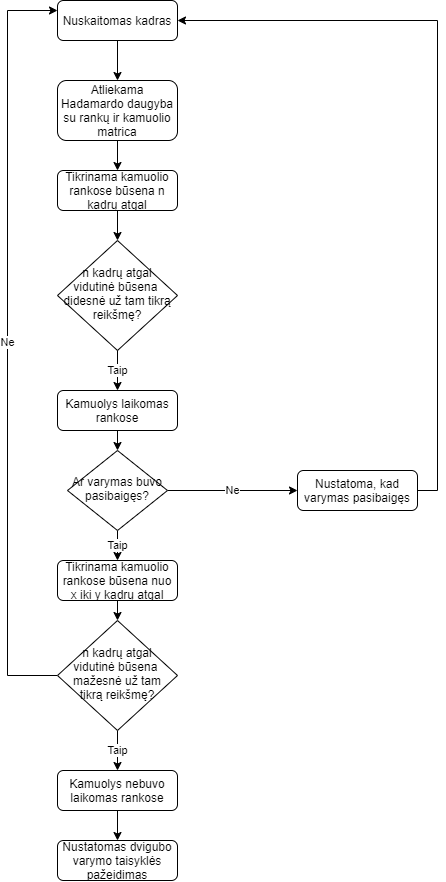
\includegraphics[scale=0.6]{img/doubledrible_algorithm}
	\caption{Dvigubo varymo taisyklės pažeidimo atpažinimo algoritmas}
	\label{img:doubledribble_algo}
\end{figure}

Varymo sustabdymą indikuoja tai, jog po varymo kamuolys buvo suimtas abejomis rankomis. Tai atpažinti, jei žaidėjas yra filmuojamas iš priekio, galima atlikus Hadamardo daugybą su išskirtomis rankų ir kamuolio sritį reprezentuojančiomis matricomis (darant prielaidą, jog jų dimensijos sutampa):

\begin{equation}\label{eq:double_dribble}
	M_{kamuolys\ rankose} = M_{kamuolys} \odot (M_{\textit{kairė\ ranka}} + M_{\textit{dešinė\ ranka}}).
\end{equation}

\ref{eq:double_dribble} lygtyje M reiškia loginę matricą, reprezentuojančią tam tikros kūno dalies sritį kadre. 

Šis būdas netinkamas tada, kai žaidėjas yra filmuojamas iš šono – tuomet spalviniais bei žmogaus pozos atpažinimo metodais neįmanoma nustatyti, kur yra žaidėjo užstojama ranka, nes jos tiesiog nesimato. Tam, kad dalinai išspręsti šią problemą, galima pasinaudoti įžvalga, jog sustabdžius varymą ir kamuolį suėmus abejomis rankomis, kamuolys bent tam tikrą laiko tarpą lieka rankose. Šis laiko tarpas yra pakankamai reikšmingas, kad būtų galima jį atpažinti apdorojant kadrus vienas po kito. 

Laiko tarpui, kai kamuolys laikomas rankose, nustatymui galima pasinaudoti 4.3.1. poskyriuje aprašytu būsenos saugojimo algoritmu. 

\section{Atlikti bandymai ir analizė}

\subsection{Įgyvendinta programinė įranga}

Aprašyti kompiuterinės regos metodai bei taisyklių atpažinimo algoritmai buvo įgyvendinti sukuriant programinę įrangą. Žaidėjo kūno dalių identifikavimui buvo pasirinktas skeleto atpažinimas neuroninio tinklo pagalba, kamuolio radimui – atpažinimas pagal spalvą. 

\begin{figure}[H]
	\centering
	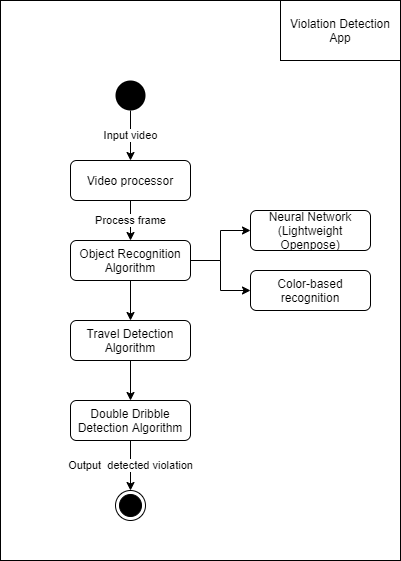
\includegraphics[scale=0.6]{img/program_architecture}
	\caption{Įgyvendintos taisyklių pažeidimo atpažinimo programinės įrangos architektūra aukštu lygmeniu}
	\label{img:program_architecture}
\end{figure}

Taip pat buvo sukurti ir įgyvendinti testavimo scenarijai, kiekviename iš jų vaizdo medžiaga yra pateikiama įgyvendintai programinei įrangai ir laukiama tam tikro rezultato, nusakančio, ar taisyklė buvo pažeista ir jei taip – kuri.  

\subsection{Atlikti bandymai}
Įgyvendinus aprašytus algoritmus, jie buvo patikrinti su paruošta vaizdo medžiaga. Šiam darbui su Sony Xperia 5 buvo nufilmuota 53 skirtingų vaizdo įrašų, atitinkančių 2 skyriuje keliamus reikalavimus. Dauguma jų filmuoti skirtingu dienos laiku, skirtingais kampais bei atstumu nuo žaidėjo. Kiekviename iš vaizdo įrašų žaidėjas pažeidžia arba dvigubo varymo taisyklę, arba žingsnių taisyklę, arba nepažeidžia nei vienos.  

Vaizdo įrašai sugrupuoti į grupes, išvardintas \ref{tab:video_groups} lentelėje.

\begin{table}[H]\footnotesize
	\centering
	\caption{Paruoštų vaizdo įrašų grupės ir jų skaičius}
	{\begin{tabular}{|p{3cm}|p{6cm}|p{3cm}|} \hline
			\textbf{Grupės nr.} & \textbf{Vaizdo įrašo apibūdinimas}  & \textbf{Vaizdo įrašų skaičius} \\
			\hline
			1  & Paprastas varymas, nepažeidžiantis taisyklių & 18 \\
			\hline
			2  & Klaidinantis veiksmas, kur žaidėjas beveik suima kamuolį, bet varo toliau, nepažeisdamas taisyklių & 6 \\
			\hline
			3  & Varymas, po kurio žaidėjas išmeta kamuolį ir jį pagauna nepažeidžiant taisyklių & 4 \\
			\hline
			4  & Žingsnių taisyklės pažeidimas & 12 \\
			\hline
			5  & Dvigubo varymo taisyklės pažeidimas kamuolį suemant į abi rankas ir tęsiant varymą & 8 \\
			\hline
			6  & Dvigubo varymo taisyklės pažeidimas kamuolį išmetant ir tęsiant varymą & 5 \\
			\hline
	\end{tabular}}
	\label{tab:video_groups}
\end{table}

\subsubsection{Pirmasis bandymas}

Pirmojo bandymo metu programinė įranga, įgyvendinanti kamuolio atpažinimą remiantis spalva, kūno dalių atpažinimą neuroninio tinklo pagalba bei abu aprašytus taisyklių pažeidimo atpažinimo algoritmus, buvo išbandyta su 53 vaizdo įrašais. Bandymo rezultatai pateikti \ref{tab:first_trial} lentelėje, o \ref{tab:first_trial_percents} lentelėje pateikti tikslumo, jautrumo bei specifiškumo procentai (laikant, jog atpažinta ne ta taisyklė yra ekvivalentu pažeidimui, kai jo nebuvo, radimui (\textit{angl.} false positive)). 

 \begin{table}[H]\footnotesize
 	\centering
 	\caption{Pirmojo bandymo atpažinimo rezultatai}
 	{\begin{tabular}{|p{3cm}|p{3cm}|p{3cm}|p{3cm}|p{2cm}|} \hline
 			\textbf{Teisingai suklasifikuota kaip taisyklių pažeidimas} & \textbf{Teisingai suklasifikuota kaip taisyklių pažeidimo nebuvimas} & \textbf{Taisyklės pažeidimas rastas, nors jo nebuvo (angl. false positive)} & \textbf{Taisyklės pažeidimas nerastas, nors jis buvo (angl. false negative)} & \textbf{Atpažinta ne ta taisyklė} \\
 			\hline
 			14  & 16    & 12    & 6    & 5   \\

 			\hline
 	\end{tabular}}
 	\label{tab:first_trial}
 \end{table}

 \begin{table}[H]\footnotesize
	\centering
	\caption{Pirmojo bandymo atpažinimo tikslumas, jautrumas bei specifiškumas}
	{\begin{tabular}{|p{5cm}|p{5cm}|p{5cm}|} \hline
			\textbf{Tikslumas} & \textbf{Jautrumas} & \textbf{Specifiškumas} \\
			\hline
			56.6\%  & 70\%    & 48.48 \%    \\
			
			\hline
	\end{tabular}}
	\label{tab:first_trial_percents}
\end{table}

\subsubsection{Antrasis bandymas}

Po pirmojo bandymo buvo pastebėta, jog dvigubo varymo taisyklių pažeidimo algoritmas yra pernelyg jautrus pokyčiams atpažindamas, kada kamuolys yra rankose. Jei kamuolio pozicija bent trumpam yra prie abiejų rankų, algoritmas iš karto laiko, jog kamuolys buvo suimtas. Antrajam bandymui buvo pakoreguoti 4.2.1 poskyryje aprašytos būsenos saugojimo skaičiavimo parametrai taip, jog nuspręsti, ar kamuolys yra tikrai laikomas rankose, būsenoje turi būti išsaugota daugiau kadrų, kada kamuolys užtikrintai buvo rankose, nei prieš tai.

Antrasis bandymas buvo atliktas su tais pačiais vaizdo įrašais, kaip ir pirmasis, tik pakoregavus algoritmo būsenos saugojimo tikrinamų kadro skaičių parametrą į didesnį. Antrojo bandymo rezultatai pateikti  \ref{tab:second_trial} bei \ref{tab:second_trial_percents} lentelėse.

\begin{table}[H]\footnotesize
	\centering
	\caption{Antrojo bandymo atpažinimo rezultatai}
	{\begin{tabular}{|p{3cm}|p{3cm}|p{3cm}|p{3cm}|p{2cm}|} \hline
			\textbf{Teisingai suklasifikuota kaip taisyklių pažeidimas} & \textbf{Teisingai suklasifikuota kaip taisyklių pažeidimo nebuvimas} & \textbf{Taisyklės pažeidimas rastas, nors jo nebuvo (angl. false positive)} & \textbf{Taisyklės pažeidimas nerastas, nors jis buvo (angl. false negative)} & \textbf{Atpažinta ne ta taisyklė} \\
			\hline
			11  & 26    & 2    & 9    & 5   \\
			\hline
	\end{tabular}}
	\label{tab:second_trial}
\end{table}

\begin{table}[H]\footnotesize
	\centering
	\caption{Antrojo bandymo atpažinimo tikslumas, jautrumas bei specifiškumas}
	{\begin{tabular}{|p{5cm}|p{5cm}|p{5cm}|} \hline
			\textbf{Tikslumas} & \textbf{Jautrumas} & \textbf{Specifiškumas} \\
			\hline
			69.81 \%  & 55\%    & 74.29 \%    \\
			
			\hline
	\end{tabular}}
	\label{tab:second_trial_percents}
\end{table}

Antrojo bandymo metu padidėjo algoritmo tikslumas bei ženkliai paaugo specifiškumas, tačiau sumažėjo jautrumas, kas indikuoja, jog nors algoritmo atpažinimas yra tikslesnis, atpažįstama mažiau tikrų pažeidimų. Taip yra todėl, kad sugriežtėjo tikrinimas, ar kamuolys yra rankose, todėl pažeidimas nėra atpažįstamas visais atvejais. 

Toliau pateikiami antrojo bandymo rezultatai, sugrupuoti pagal vaizdo įrašų grupes.

\begin{table}[H]\footnotesize
	\centering
	\caption{Antrojo bandymo atpažinimo rezultatai pagal vaizdo įrašų grupes}
	{\begin{tabular}{|p{3cm}|p{3cm}|p{3cm}|p{3cm}|} \hline
			\textbf{Vaizdo įrašo grupė} & \textbf{Įrašų kiekis} & \textbf{Suklasifikuota teisingai} & \textbf{Suklasifikuota neteisingai} \\
			\hline
			1  & 18    & 16    & 2    \\
			\hline
			2  & 6    & 5  & 1     \\
			\hline
			3  & 4    & 4   & 0    \\
			\hline
			4  & 12    & 4  & 8     \\
			\hline
			5  & 8    & 5  & 3     \\
			\hline
			6  & 5    & 3  & 2     \\
			\hline
	\end{tabular}}
	\label{tab:recognizion_results_grouped}
\end{table}

Iš 11 lentelės matyti, jog mažiausiai teisingai suklasifikuoti vaizdo įrašai, kuriuose yra žingsnių taisyklės pažeidimas.  

\subsubsection{Trečiasis ir ketvirtas bandymai}

Trečiasis ir ketvirtasis bandymai buvo atlikti siekiant patikrinti kiekvieną taisyklės pažeidimo algoritmą individualiai, t.y. kiekvieno bandymo metu vaizdo medžiaga patikrinta arba tik su dvigubo varymo, arba tik su žingsnių taisyklės pažeidimo atpažinimo algoritmu. Lyginant su prieš tai atliktais bandymais, kiekvieno bandymo metu testai buvo pamodifikuoti, jog vienos taisyklės pažeidimo atpažinimą, testas nesitikėtų, kad bus atpažinti kitos taisyklės pažeidimai. 

Trečiojo bei ketvirtojo bandymo rezultatai pateikiami \ref{tab:third_trial}, \ref{tab:fourth_trial}, \ref{tab:third_trial_percents}, \ref{tab:fourth_trial_percents}, \ref{tab:third_trial_recognizion_results_grouped} bei \ref{tab:fourth_trial_recognizion_results_grouped} lentelėse. 

\begin{table}[H]\footnotesize
	\centering
	\caption{Trečiojo bandymo žingsnių taisyklės pažeidimo atpažinimo rezultatai}
	{\begin{tabular}{|p{3cm}|p{3cm}|p{3cm}|p{2cm}|} \hline
			\textbf{Teisingai suklasifikuota kaip taisyklių pažeidimas} & \textbf{Teisingai suklasifikuota kaip taisyklių pažeidimo nebuvimas} & \textbf{Taisyklės pažeidimas rastas, nors jo nebuvo (angl. false positive)} & \textbf{Taisyklės pažeidimas nerastas, nors jis buvo (angl. false negative)} \\
			\hline
			4  & 40    & 1    & 8      \\
			\hline
	\end{tabular}}
	\label{tab:third_trial}
\end{table}

\begin{table}[H]\footnotesize
	\centering
	\caption{Ketvirtojo bandymo dvigubo varymo taisyklės pažeidimo atpažinimo rezultatai}
	{\begin{tabular}{|p{3cm}|p{3cm}|p{3cm}|p{2cm}|} \hline
			\textbf{Teisingai suklasifikuota kaip taisyklių pažeidimas} & \textbf{Teisingai suklasifikuota kaip taisyklių pažeidimo nebuvimas} & \textbf{Taisyklės pažeidimas rastas, nors jo nebuvo (angl. false positive)} & \textbf{Taisyklės pažeidimas nerastas, nors jis buvo (angl. false negative)} \\
			\hline
			7  & 32    & 8    & 6   \\
			\hline
	\end{tabular}}
	\label{tab:fourth_trial}
\end{table}

\begin{table}[H]\footnotesize
	\centering
	\caption{Trečiojo bandymo rezultatų tikslumas, jautrumas bei specifiškumas}
	{\begin{tabular}{|p{5cm}|p{5cm}|p{5cm}|} \hline
			\textbf{Tikslumas} & \textbf{Jautrumas} & \textbf{Specifiškumas} \\
			\hline
			83.02 \%  & 33 \%    & 97.56 \%    \\
			
			\hline
	\end{tabular}}
	\label{tab:third_trial_percents}
\end{table}

\begin{table}[H]\footnotesize
	\centering
	\caption{Ketvirtojo bandymo rezultatų tikslumas, jautrumas bei specifiškumas}
	{\begin{tabular}{|p{5cm}|p{5cm}|p{5cm}|} \hline
			\textbf{Tikslumas} & \textbf{Jautrumas} & \textbf{Specifiškumas} \\
			\hline
			73.58 \%  & 53.8 \%    & 80 \%    \\
			
			\hline
	\end{tabular}}
	\label{tab:fourth_trial_percents}
\end{table}

\begin{table}[H]\footnotesize
	\centering
	\caption{Trečiojo bandymo žingsnių taisyklės pažeidimo atpažinimo rezultatai pagal vaizdo įrašų grupes}
	{\begin{tabular}{|p{3cm}|p{3cm}|p{3cm}|p{3cm}|} \hline
			\textbf{Vaizdo įrašo grupė} & \textbf{Įrašų kiekis} & \textbf{Suklasifikuota teisingai} & \textbf{Suklasifikuota neteisingai} \\
			\hline
			1  & 18    & 17    & 1    \\
			\hline
			2  & 6    & 5  & 1     \\
			\hline
			3  & 4    & 4   & 0    \\
			\hline
			4  & 12    & 4  & 8     \\
			\hline
			5  & 8    & 8  & 0     \\
			\hline
			6  & 5    & 5  & 0    \\
			\hline
	\end{tabular}}
	\label{tab:third_trial_recognizion_results_grouped}
\end{table}

\begin{table}[H]\footnotesize
	\centering
	\caption{Ketvirtojo bandymo dvigubo varymo taisyklės pažeidimo atpažinimo rezultatai pagal vaizdo įrašų grupes}
	{\begin{tabular}{|p{3cm}|p{3cm}|p{3cm}|p{3cm}|} \hline
			\textbf{Vaizdo įrašo grupė} & \textbf{Įrašų kiekis} & \textbf{Suklasifikuota teisingai} & \textbf{Suklasifikuota neteisingai} \\
			\hline
			1  & 18    & 16    & 2    \\
			\hline
			2  & 6    & 6  & 0     \\
			\hline
			3  & 4    & 4   & 0    \\
			\hline
			4  & 12    & 5  & 7     \\
			\hline
			5  & 8    & 5  & 3     \\
			\hline
			6  & 5    & 2  & 3     \\
			\hline
	\end{tabular}}
	\label{tab:fourth_trial_recognizion_results_grouped}
\end{table}

Lyginant 12 bei 13 lentelę pastebima, jog žingsnių taisyklės pažeidimo atpažinimo algoritmas yra griežtesnis, nei dvigubo varymo atpažinimo algoritmas, t.y. jis linkęs mažiau rasti teigiamų atvejų, bet tuo pačiu ir mažiau klaidingai teigiamų. Toks algoritmas, nors ir praleidžiantis ne mažą dalį nusižengimų, labai retai juos atpažintų neteisingai, taip nepelnytai nubausdamas žaidėjus bei sustabdydamas žaidimo tėkmę. 

Žingsnių taisyklės pažeidimo sąlygos yra griežtesnės, nei dvigubo varymo (t.y. daugiau nei 2 žingsniai per tam tikrą intervalą, kuris gali trūkinėti, taip pat – žingsnių skaičiavimo priklausomumas nuo idealių žingsniavimo sąlygų), todėl žingsnių taisyklės pažeidimas yra pastebimas rečiau. Praktikoje žingsnių taisyklės pažeidimas taip pat yra pastebimas gan retai \cite{SiglerK}, trečiojo bandymo metu pasiektas jautrumas yra didesnis, nei vidutinis teisėjų tikruose NBA žaidimuose. 

\subsubsection{Penktasis bandymas}

Penktajam bandymui buvo paruošta papildomi 33 vaizdo įrašai. Jie filmuoti aukštesne raiška, nei praeituose bandymuose bei kita kamera (Xiaomi Redmi 8 Pro su 4K raiškos kamera), taip pat kitoje vietoje, tad vaizdo įrašų fonas kitoks, nei praeituose bandymuose – juose mažiau trukdžių. Taip pat buvo bandoma filmuoti kuo arčiau, kad atpažinimo algoritmams būtų kuo lengviau atpažinti rankas, kojas bei kamuolį. 12 iš vaizdo įrašų atliekami dvigubo varymo taisyklės pažeidimai, 11 – žingsnių taisyklės pažeidimai, 10 – jokių pažeidimų nėra. 

Kaip ir praeituose bandymuose, skaičiuojant tikslumą, jautrumą bei specifiškumą, vaizdo įrašai, suklasifikuoti ne ta taisykle, kuria turėtų, laikomi klaidingai teigiamais. 

\begin{table}[H]\footnotesize
	\centering
	\caption{Penktojo bandymo dvigubo varymo taisyklės pažeidimo atpažinimo rezultatai}
	{\begin{tabular}{|p{3cm}|p{3cm}|p{3cm}|p{2cm}|} \hline
			\textbf{Teisingai suklasifikuota kaip taisyklių pažeidimas} & \textbf{Teisingai suklasifikuota kaip taisyklių pažeidimo nebuvimas} & \textbf{Taisyklės pažeidimas rastas, nors jo nebuvo (angl. false positive)} & \textbf{Taisyklės pažeidimas nerastas, nors jis buvo (angl. false negative)} \\
			\hline
			10  & 10    & 4    & 3   \\
			\hline
	\end{tabular}}
	\label{tab:fifth_trial}
\end{table}

\begin{table}[H]\footnotesize
	\centering
	\caption{Trečiojo bandymo rezultatų tikslumas, jautrumas bei specifiškumas}
	{\begin{tabular}{|p{5cm}|p{5cm}|p{5cm}|} \hline
			\textbf{Tikslumas} & \textbf{Jautrumas} & \textbf{Specifiškumas} \\
			\hline
			74.07 \%  & 76.92 \%    & 71.43 \%    \\
			
			\hline
	\end{tabular}}
	\label{tab:fifth_trial_percents}
\end{table}

Šie rezultatai geresni, nei praeituose bandymuose, nes paruoštos vaizdo medžiagos turinys buvo labiau kontroliuojamas, t.y. filmuojama stengiantis rankas, kojas bei kamuolį padaryti kuo labiau matomais.

\subsection{Klaidingų bandymų rezultatų analizė}

Atlikus visus aprašytus bandymus buvo pastebėta keletas dėsningumų, lemiančių klaidingus rezultatus. Dalis jų buvo pataisyti bandymų eigoje, perskaičiuojant rezultatus iš naujo.

\subsubsection{Fono trukdžiai}

Atliekant bandymus pastebėta, jog dalyje vaizdo įrašų matomas fonas, kuriame yra smulkus, tokios pačios spalvos, kaip ir kamuolys, objektas. Dėl šio objekto atpažinimo algoritmas teisingai neatpažindavo kamuolio, kas lemdavo tai, jog žingsnių taisyklių pažeidimas nebuvo atpažintas. 

Šis trukdis darė įtaką trijų žingsnių taisyklės pažeidimo atpažinimui trijuose 4 grupės vaizdo įrašuose, jie atpažinti kaip nepažeidžiantys taisyklių. 

\subsubsection{Atpažinimo pagal spalvą netikslumas}

Viename vaizdo įraše, kuriame atliekamas žingsnių taisyklės pažeidimas atliekant pirmuosius bandymus pastebėta, jog kamuoliui nutolus nuo kameros bei žaidėjui nuėjus į tamsesnę vietą kamuolys nebebuvo atpažintas, kadangi jo HSV spalva išėjo iš iš anksto nustatytų rėžių.  

\subsubsection{Kamuolio suėmimo atpažinimo metodo neefektyvumas}

Dvigubo varymo taisyklės pažeidimo atpažinimo metu tikrinama, ar kamuolys yra laikomas rankose atliekant Hadamardo daugybą su kamuolį bei rankas reprezentuojančiomis matricomis. Tačiau toks būdas yra neefektyvus, ypač tikrinant, ar laikoma abejose rankose. Pastebėta, jog varant kamuolį viena ranka jis dažnai uždengia kitą ranką, dėl ko algoritmas tai nustato kaip laikymą abejose rankose, kadangi objektų atpažinimo metodai yra dvimačiai, neatpažįstantys erdvės gylio skirtumų.

Buvo bandoma keisti laikymo rankose būsenos parametrus padidinant reikiamų kadrų, kuriuose kamuolys yra abejose rankose, kiekį, tačiau tai ženkliai apsunkino dvigubo varymo taisyklės pažeidimo atpažinimą, tikslumui nukrentant iki 20 proc.

\begin{figure}[H]
	\centering
	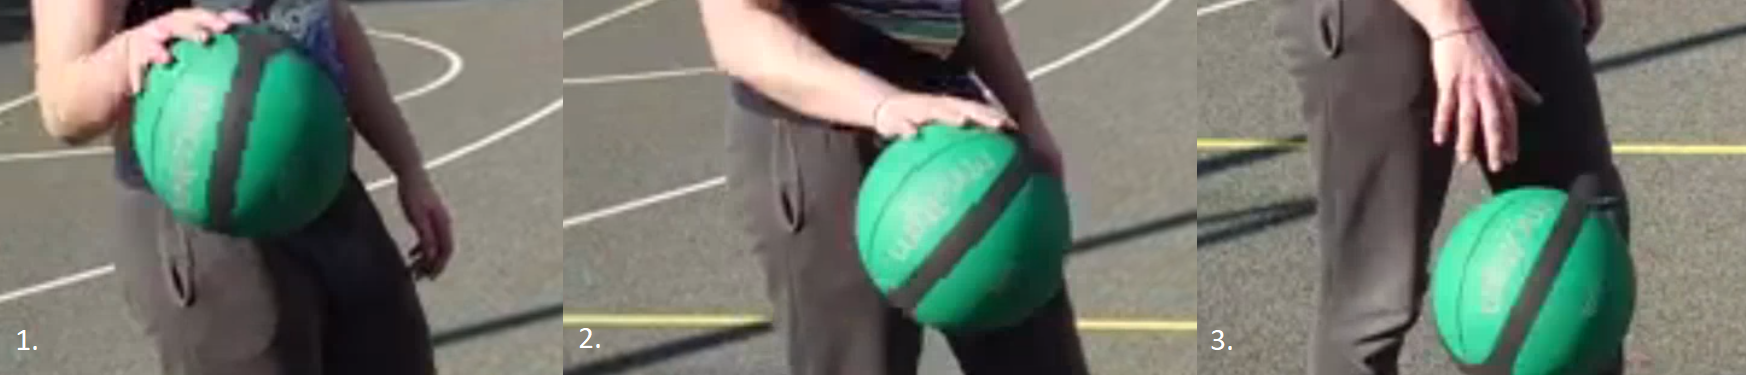
\includegraphics[scale=0.3]{img/double_dribble_fault.png}
	\caption{ Kamuolio varymo kadrai }
	\label{img:double_dribble_fault}
\end{figure}

\ref{img:double_dribble_fault} paveikslėlyje matyti, kad nors 1 ir 3 kadre akivaizdu, jog kamuolys nėra laikomas abejose rankose, tą patį nustatyti 2 kadre galime tik žinodami kontekstą, pvz., alkūnės linkį, kamuolio atstumą nuo rankos ir pan.  

Dėl šio neefektyvumo bent 6 vaizdo įrašai 4 grupėje klaidingai klasifikuoti kaip pažeidžiantys dvigubo varymo taisyklę, algoritmui nusprendus, kad kamuolys buvo suimtas ir vėl paleistas. 

\subsubsection{Neuroninio tinklo atpažinimo netikslumai}

Atliekant bandymus pastebėta, jog šiame darbe naudotas neuroninio tinklo modelis turi sunkumų atpažįstant koją, kai viena koja pridengia kitą. Dėl šių netikslumų algoritmas, skaičiuojantis, kada atliktas žingsnis, tampa netikslus, kadangi jis priklauso nuo to, kiek pėdų kontūrų pavyksta atrasti. Neuroniniui tinklui bent vieną kadrą neatradus kažkurios pėdos pozicijos, žingsnis gali būti neatpažintas. 

\begin{figure}[H]
	\centering
	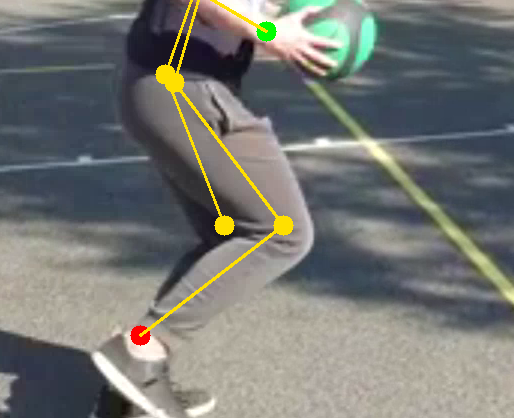
\includegraphics[scale=0.6]{img/neural_network_fault.png}
	\caption{ Neuroninio tinklo kojos atpažinimo netikslumas }
	\label{img:neural_network_fault}
\end{figure}

Šis netikslumas turėjo įtaką bent 4 vaizdo įrašams, kuriuose atliekamas žingsnių taisyklės pažeidimas. Pastebėta, kad šiek tiek sumažėjo klaidingai neigiamų rezultatų dvigubai padidinus neuroninio tinklo įvesties dydį, tačiau apdorojimo laikas bei naudojami kompiuteriniai resursai išaugo tiek, jog tolimesnių bandymų su daugiau vaizdo medžiagos atlikti nebepavyko.

Kitas gan svarbus netikslumas – kūno dalių pozicijos. Šiame darbe naudotas žmogaus skeletą atpažįstantis neuroninis tinklas nurodo ne pačių rankų ar pėdų pozicijas, bet riešo bei kulkšnies. Tai apsunkina atpažinimą, kai siekiama nustatyti, ar kamuolys yra laikomas bent vienoje rankoje. Beveik visuose vaizdo įrašuose pastebėta, jog neuroninio tinklo rasta riešo pozicija kai kuriuose kadruose buvo per toli nuo kamuolio, tad algoritmas nustatydavo, jog kamuolys nėra laikomas rankose, dėl ko vienu atveju buvo nutraukiamas žingsnių skaičiavimas. 

\subsection{Galutiniai bandymų rezultatai}

Šiame poskyriuje pateikiami galutiniai rezultatai, programinę įrangą patikrinus su visais 86 vaizdo įrašais. 

\begin{table}[H]\footnotesize
	\centering
	\caption{Galutiniai dvigubo varymo taisyklės pažeidimo atpažinimo rezultatai}
	{\begin{tabular}{|p{3cm}|p{3cm}|p{3cm}|p{3cm}|p{2cm}|} \hline
			\textbf{Teisingai suklasifikuota kaip taisyklių pažeidimas} & \textbf{Teisingai suklasifikuota kaip taisyklių pažeidimo nebuvimas} & \textbf{Taisyklės pažeidimas rastas, nors jo nebuvo (angl. false positive)} & \textbf{Taisyklės pažeidimas nerastas, nors jis buvo (angl. false negative)} & \textbf{Atpažinta ne ta taisyklė} \\
			\hline
			21  & 36    & 2    & 12  &  9 \\
			\hline
	\end{tabular}}
	\label{tab:final_results}
\end{table}

\begin{table}[H]\footnotesize
	\centering
	\caption{Galutinių rezultatų tikslumas, jautrumas bei specifiškumas}
	{\begin{tabular}{|p{5cm}|p{5cm}|p{5cm}|} \hline
			\textbf{Tikslumas} & \textbf{Jautrumas} & \textbf{Specifiškumas} \\
			\hline
			71.25 \%  & 63.64 \%    & 76.60 \%    \\
			\hline
	\end{tabular}}
	\label{tab:final_results_percents}
\end{table}

\sectionnonum{Rezultatai}

Šio darbo metu buvo:

\begin{enumerate}
	\item išnagrinėti kompiuterinės regos metodai, skirti žmogaus bei kamuolio atpažinimui – segmentavimas pagal spalvą, atpažinimas remiantis paveikslėlio skirtumais bei atpažinimas neuroniniu tinklu,
	\item atliktas eksperimentas lyginantis nagrinėtų kompiuterinės regos metodų atpažinimo spartą bei tikslumą juos pritaikant žingsnių skaičiavimo algoritmui, 
	\item apibrėžti krepšinio taisyklių pažeidimo algoritmai, pritaikantys nagrinėtus kompiuterinės regos metodus:
	\begin{enumerate}
		\item apibrėžtas žingsnių taisyklės pažeidimo atpažinimo algoritmas,
		\item apibrėžtas dvigubo varymo taisyklės pažeidimo atpažinimo algoritmas;
	\end{enumerate}
	\item aprašyti algoritmai bei kompiuterinės regos pritaikyti sukūrus juos įgyvendinančią programinę įrangą,
	\item programinė įranga išbandyta su vaizdo medžiaga. Žingsnių bei dvigubo varymo taisyklių pažeidimai buvo nustatyti 71.25\% tikslumu, jautrumas 63.64\%, specifiškumas 76.60\%.
\end{enumerate}

\sectionnonum{Išvados}

Darbo metu pasiektos šios išvados:

\begin{enumerate}
	\item pateiktieji taisyklių pažeidimo atpažinimo algoritmai, OpenPose neuroninio tinklo modelis bei kamuolio atpažinimas segmentavimo metodu yra tinkami siekiant taisyklių pažeidimus nustatyti bent 70 procentų tikslumu;
	\item atpažinimo remiantis spalva metodai nepasiekia tokio tikslumo, kaip atpažinimas naudojantis neuroniniu tinklu, tačiau yra spartesni. Šių metodų teikiamas tikslumas kenčia dėl nuolat besikeičiančio apšvietimo vaizdo įrašuose;
	\item atpažinimas remiantis kadrų skirtumais yra tinkamas siekiant atpažinti judesį, pavyzdžiui, skaičiuojant atliktus žingsnius. Šis būdas yra greičiausias iš nagrinėtų, tačiau tuo pačiu ir netiksliausias;
	\item dvigubo varymo taisyklės pažeidimo algoritmas yra mažiau tikslus, nei žingsnių taisyklės, tačiau jautresnis, kadangi įvykus netikslumui atpažinimo metu griežtesnės žingsnio atpažinimo sąlygos nėra tenkinamos, tuo tarpu dvigubo varymo sąlygos yra tenkinamos dažniau, nei tikėtasi. Tai sąlygojo, jog dalis vaizdo įrašų algoritmo buvo suklasifikuoti kaip klaidingai teigiami.
	\item taisyklių pažeidimo atpažinimą neigiamai veikia fono trukdžiai, apšvietimo bei objektų nuotolio pokyčiai, neuroninio tinklo netikslumai atpažįstant žmogaus skeletą;
	\item aprašytas kamuolio laikymo abejose rankose nustatymas gali sąlygoti klaidingai teigiamus rezultatus dėl papildomos informacijos apie rankų poziciją trimatėje erdvėje trūkumo.
\end{enumerate}

Toliau pateikiamos rekomendacijos bei tolimesni darbai.

\begin{enumerate}
	\item Siūloma išnagrinėti ne žmogaus skeletą atpažįstančius neuroninių tinklų modelius, bet kūno dalių segmentavimo neuroninius tinklus, siekiant išgauti tikslesnes kūno dalių pozicijas.
	\item Tokiais atvejais, kai kūno dalių, pvz., pėdų neuroninis tinklas atpažinti negali, siūloma sekti kūno dalių pozicijų pokyčius ir nustatyti jų galimą buvimo vietą į ateitį. Taip bus dalinai apsisaugoma nuo atvejų, kai nežinoma, kurioje vietoje yra žaidėjo koja ar ranka.
	\item Kamuolio atpažinimas spalva yra svarbus trūkumas, kadangi ne tik tokiu atveju vaizdo medžiaga turi būti iš anksto paruošta, joje neturi būti jokių tos pačios spalvos trukdžių, bet ir spalvos kintamumas lemia tai, jog objektas gali likti neatpažintas. 
	\item Taisyklių pažeidimo algoritmai galėtų būti lankstesni ir praktiškesni, siekiant sumažinti klaidingų neigiamų atpažinimų skaičių. Šiame darbe apibrėžtas žingsnių taisyklės pažeidimo algoritmas labiausiai veiksmingas tada, kai į žaidėją žiūrima iš šono, o dvigubo varymo – tada, kai į žaidėją žiūrima iš priekio. 
\end{enumerate}

\printbibliography[heading=bibintoc,title=Šaltiniai]  % Šaltinių sąraše nurodoma panaudota
% literatūra, kitokie šaltiniai. Abėcėlės tvarka išdėstomi darbe panaudotų
% (cituotų, perfrazuotų ar bent paminėtų) mokslo leidinių, kitokių publikacijų
% bibliografiniai aprašai. Šaltinių sąrašas spausdinamas iš naujo puslapio.
% Aprašai pateikiami netransliteruoti. Šaltinių sąraše negali būti tokių
% šaltinių, kurie nebuvo paminėti tekste. Šaltinių sąraše rekomenduojame
% necituoti savo kursinio darbo, nes tai nėra oficialus literatūros šaltinis.
% Jei tokių nuorodų reikia, pateikti jas tekste.


\appendix  % Priedai
% Prieduose gali būti pateikiama pagalbinė, ypač darbo autoriaus savarankiškai
% parengta, medžiaga. Savarankiški priedai gali būti pateikiami ir
% kompaktiniame diske. Priedai taip pat numeruojami ir vadinami. Darbo tekstas
% su priedais susiejamas nuorodomis.

\section{Sukurtos programinės įrangos kodo nuoroda}
https://github.com/LukasCed/basketball-rules-violation-thesis

\section{Vaizdo įrašai, naudoti žingsnių skaičiavimui}
https://drive.google.com/drive/folders/13BI-eH62bwaUmMGrrUmE752j4UVvtUKU?usp=sharing

\section{Vaizdo įrašai, naudoti programinės įrangos bandymams}
https://drive.google.com/drive/folders/1DhaJ8jNA3UDzxzZMwFsx9E0gr7lm0GAk?usp=sharing

\end{document}